\documentclass[12pt]{article}
\usepackage[utf8]{inputenc}
\usepackage{amsmath}
\usepackage{amsfonts}
\usepackage{amssymb}
\usepackage{graphicx}
\usepackage{hyperref}
\usepackage{geometry}
\geometry{a4paper, margin=2cm}
\usepackage{tabularx}
\usepackage{enumitem}
\usepackage{setspace}  % For line spacing control
\usepackage{tocloft}   % For Table of Contents formatting
\usepackage{float}     % For [H] figure/table placement
\usepackage{placeins}  % For \FloatBarrier

% Set 1.5 line spacing for main text
\onehalfspacing

% Set font to Times New Roman (if available)
\usepackage{times}

% Graphics path for figures
\graphicspath{{figures/}}

% Set up word count command using texcount (requires -shell-escape)
% \newcommand\wordcount{\input{|"texcount -1 -sum 'TE Classification.tex'"}}
\newcommand\wordcount{7,261}

\begin{document}

% ============ TITLE PAGE ============
\begin{titlepage}
    \centering
    \vspace*{2cm}
    
    % Title
    {\LARGE\bfseries Machine Learning a Transposable Element Classifier\par}
    
    \vspace{3cm}
    
    % Author name
    {\Large Yingrui Yang\par}
    
    \vspace{3cm}
    
    % Supervisor information
    {\large 
    Supervisor: Richard Durbin\par
    \vspace{0.5cm}
    Day-to-day Supervisors: Pio Sierra, Hadi Khan\par
    }
    
    \vfill
    
    % Word count statement
    {\normalsize This thesis contains approximately \wordcount\ words.\par}
    
    \vspace{1cm}
    
\end{titlepage}

% ============ DECLARATION PAGE ============
\newpage
\thispagestyle{empty}

\vspace*{1cm}

\begin{center}
    {\Large\bfseries Declaration\par}
\end{center}

\vspace{1cm}

\noindent\textbf{Name:} Yingrui Yang

\vspace{0.5cm}

\noindent\textbf{College:} Emmanuel College

\vspace{0.5cm}

\noindent\textbf{Title:} Machine Learning a Transposable Element Classifier

\vspace{1.5cm}

\noindent I understand the University's definition of plagiarism. I declare that, in accordance with Discipline regulation 6, this dissertation is entirely my own work except where otherwise stated, either in the form of citation of published work, or acknowledgement of the source of any unpublished material.

\vspace{1.5cm}

\noindent The project is purely computational and does not involve any wet lab experiments. The models were either trained locally or on CSD3 in the Western Cambridge Data Center, with the access provided by the research group. 

\vspace{2cm}

\noindent\textbf{Signature:} \hrulefill

\vspace{1cm}

\noindent\textbf{Date:} \hrulefill

% ============ BLIND GRADING NUMBER PAGE ============
\newpage
\thispagestyle{empty}

\vspace*{\fill}
\begin{center}
    {\fontsize{24.88}{34}\selectfont\bfseries Part III project report 6506D\par}
\end{center}
\vspace*{\fill}

% ============ SUMMARY ============
\newpage
\section*{Summary}
\addcontentsline{toc}{section}{Summary}

Transposable elements (TEs) are repeated [sequences / structural units] that require computational classification for genomic analysis. Existing tools rely on alignment and manual curation, limiting scalability. This project develops deep learning classifiers leveraging large-scale TE catalogs from the Vertebrate Genomes Project.

The core contribution is a hybrid convolutional-graph neural network (CNN+GNN) architecture that achieves 98.2\% accuracy on three-class discrimination (DNA transposons / LTR retrotransposons / LINEs) and 89.3\% accuracy on superfamily-level classification across 23 families. The hybrid design fuses local sequence motifs (CNN branch, 66\% weight) with global k-mer composition (GNN branch, 34\% weight), with learned attention gating that dynamically emphasizes features conditioned on input. This attentional fusion outperforms single-modality baselines and provides interpretable weighting of feature types.

\iffalse
Systematic analysis identified key computational phenomena: (1) superfamily classification is significantly more prone to overfitting than class-level discrimination (0.127 vs. 0.016 test gaps in v4.2), requiring early stopping and species hold-out validation; (2) k-mer composition alone achieves 85\% macro F1 for class discrimination, indicating that transposition mechanism is intrinsically separable; (3) gradient-based saliency analysis reveals that well-classified sequences concentrate saliency at biologically canonical regions (TIR boundaries for DNA, poly-A motifs for LINEs), while misclassifications scatter saliency diffusely; (4) unsupervised contrastive learning recovers 82\% of supervised clustering performance without labels, demonstrating strong self-supervised structure in raw TE sequences.

External benchmarking on three held-out species (zebra finch, platypus, alligator) reveals lineage-dependent domain shift: models trained on mammalian/reptilian sequences transfer well to platypus (73.8\% class accuracy) but degrade substantially on avian genomes (33.3\% for zebra finch), indicating that TE features are phylogenetically taxon-specific. This finding motivates future work on domain adaptation and multi-lineage pretraining.

Implementation on GPU clusters achieves inference latency of 15 $\mu$s per sequence (A100), enabling genome-scale deployment. Quantization to INT8 reduces model size 3.9$\times$ with negligible accuracy loss, enabling edge deployment.
\fi

% ============ TABLE OF CONTENTS ============
\newpage
\tableofcontents

% ============ LIST OF ABBREVIATIONS ============
\newpage
\section*{List of Abbreviations}
\addcontentsline{toc}{section}{List of Abbreviations}

\begin{tabular}{ll}
    TE & Transposable Element \\
    DNA & Deoxyribonucleic Acid \\
    CNN & Convolutional Neural Network \\
    GNN & Graph Neural Network \\
    TIR & Terminal Inverted Repeat \\
    LTR & Long Terminal Repeat \\
    LINE & Long Interspersed Nuclear Element \\
    SINE & Short Interspersed Nuclear Element \\
    RC & Reverse Complement \\
    GELU & Gaussian Error Linear Unit \\
    AUROC & Area Under the Receiver Operating Characteristic Curve \\
    AUPRC & Area Under the Precision-Recall Curve \\
    QAT & Quantization-Aware Training \\
    INT8 & 8-bit Integer \\
    FP16/FP32 & 16/32-bit Floating Point \\
    CUDA & Compute Unified Device Architecture \\
    VGP & Vertebrate Genomes Project \\
    UMAP & Uniform Manifold Approximation and Projection \\
    SupCon & Supervised Contrastive Learning \\
\end{tabular}

\iffalse

%% Supervisor's plan for project - to be used as a basis for writing the thesis, but not to be included in the final document

Transposable elements (TEs) are kilobase-scale segments of DNA that insert new copies of themselves in the genome, generating over time large families of interspersed repeats (ref 1). Some of these are autonomous, themselves encoding the proteins needed to mobilise themselves, but others are non-autonomous, needing an active autonomous element to move. Our group with Prof. Karam Teixeira’s is studying the co-evolution of TE families and subfamilies with eukaryote genomes. Although we have increasingly good methods to identify TE families in new genome sequences, classifying them correctly is not a solved problem. In particular it is frequently difficult to correctly identify non-autonomous element subtypes and assign them to their driver elements. Current methods rely on detection of a set of features, with manual curation, but recently machine learning methods have been explored. In this project the student will take advantage of very large sets of TEs found using our new detection approach Pantera (ref 2), to build better classifiers using novel machine learning approaches, for example using DNA and protein foundation models and unsupervised learning to identify new families, and exploring new approaches to associate non-autonomous sequences to their drivers. One goal is to build generative models of TE sequences that encode information not captured by classic sequence alignment.

1. Wells JN, Feschotte C (2020) A Field Guide to Eukaryotic Transposable Elements. Annu Rev Genet. 54:539-561. https://doi.org/10.1146/annurev-genet-040620-022145 

2. Sierra P, Durbin R (2024) Identification of transposable element families from pangenome polymorphisms. Mobile DNA. 15:13. https://doi.org/10.1186/s13100-024-00323-y 

3. Balamurugan R, Mohite S, Raja SP (2023) Protein Sequence Classification Using Bidirectional Encoder Representations from Transformers (BERT) Approach. SN COMPUT. SCI. 4:481. https://doi.org/10.1007/s42979-023-01980-1 

4. David KT, Halanych KM (2023) Unsupervised Deep Learning Can Identify Protein Functional Groups from Unaligned Sequences, Genome Biology and Evolution, 15:evad084, https://doi.org/10.1093/gbe/evad084 

\fi

\iffalse

%% This is NOT the interium report. I could not find the original document, but this is a very relevant email and contains some high-level summaries of the work done by the time. Again, just for reference and not to be included in the final document.

CNN Tower Model (v3)

This is an update to the models I trained before the vacation, with the tower-based CNN network and RC-invariance via fusion. The model generally goes through three CNN layers with kernel sizes 7, 15, 21 to capture difference motifs, and the results are put into attention layer. The model currently has a binary head to deal with transposase vs None and a multi classification head (among 7 families since I'm ruling out all the families with fewer then 100 samples). 

I'm getting pretty decent results, with 91.3% accuracy and 0.87 Macro F1 on the binary head, and 94.4% accuracy and 0.90 Macro F1 on the multi head. Please see the confusion matrix as attached. The model performs especially well on DNA/hAT (F1=0.98) and TcMar-Tc1 (F1=0.97), while DNA/CMC remains challenging (F1=0.76), likely due to limited training samples.

I'm placing the raw sequences at random positions within a 40,000 bp window during training. Interestingly, the model learned to predict sequence length with high accuracy (correlation 0.94, MAE ~1kb), though absolute boundary positions remain difficult to localise.

CNN Tower + k-mer GNN Hybrid Model (v4)

As previously discussed, I experimented with combining a windowed k-mer GNN to help the model learn compositional patterns across the sequence. The standalone k-mer GNN does not perform as well on its own as it tends to confuse superfamilies within the DNA class since they share similar k-mer compositions. However, it provides useful complementary information, so I combined both approaches using attention-based fusion.

In the best trained epoch, the attention fusion weights settled at approximately CNN: 40% / GNN: 60%, but this proportion is quite stable at the late stage of training. The hybrid model doesn't outperform v3 on superfamily classification but is slightly better at the binary head. 

Model using the full label set (v5, in progress)

The previous models were trained with Pio's 2025-12-15 feature set, which labels over 92% sequences as "None" (no transposase detected). However, the FASTA headers themselves contain more detailed class labels (e.g., LTR/Gypsy, LINE/L1). I'm now training a model on this fuller label set, which may improve the binary classification by leveraging the richer supervision signal. 

Interim Report

Finally, regarding the interim report, I've just realised the deadline is Jan 15 and that supervisor and student need to submit separate reports. I apologise for the late notice on this. I'll be back in Cambridge on Tuesday (Jan 13), so I hope there will be enough time to complete it. Please let me know if you have any guidance or templates I should follow.

\fi

\iffalse

%% This is another quote from email. The first feature set for TIR is the starting point of the project, and the second feature set includes the classification labels for only the DNA elements, while everything else are labeled as "None". It is important to clarify that in the model files I was writing "Transposase vs None" for the second model, but it is not exactly correct since the "None" class includes all non-DNA elements, not just the ones without transposase. 

That looks good, but I am a little confused by the “Transposase vs None” model. Do you mean the first feature table? If so that is about presence/absence of TIR elements, the inverted repeats at the edges of the sequence.

If instead you mean “anything not none vs none” in the second table, that would put together all elements classified as DNA elements, but not all of them would have a transposase, so that is not what the model would be detecting.

\fi

% ============ INTRODUCTION ============
\newpage
\section{Introduction}

\subsection{Computational Challenges in Sequence Classification}

Automated classification of biological sequences is a fundamental problem in computational biology. Traditional approaches employ sequence alignment to reference databases and hand-curated pattern matching, which are inherently limited by the coverage and quality of reference libraries. These methods scale poorly with dataset size and fail when encountering divergent variants or novel families.

Deep learning has emerged as an alternative paradigm for sequence classification \cite{lecun2015deep,goodfellow2016deep}. Convolutional neural networks (CNNs) naturally capture local patterns through learned convolutional kernels, while graph neural networks (GNNs) aggregate global properties through message passing \cite{kipf2016semi,hamilton2017inductive}. The question addressed in this project is whether hybrid architectures combining these modalities can outperform single-branch approaches on a challenging real-world classification task.

\iffalse
\subsection{Transposable Elements as a Model Problem}

[Transposable elements (TEs) are kilobase-scale DNA segments that [insert / replicate / move] within genomes. Three major [mechanisms: (1) DNA transposons (cut-and-paste), (2) LTR retrotransposons, (3) LINEs (non-LTR retrotransposons).] TE families exhibit [biological properties: low sequence identity within families, mechanisms with distinct structural signatures].

The classification problem has three computational layers: (1) *coarse level*: distinguish transposition mechanisms (DNA vs. retrotransposon), based on [structural features: TIRs vs. LTRs vs. poly-A]; (2) *superfamily level*: assign to functional families (80+ known superfamilies), based on [conserved motifs]; (3) *rare-variant level*: identify novel subfamilies or assembly artifacts. Standard alignment-based tools handle layer 1 reliably but falter at layers 2--3.

The Vertebrate Genomes Project (VGP) has generated a large-scale TE catalog (140k+ sequences) through Pantera, a detection method that identifies TEs from pangenome polymorphisms. This dataset enables supervised learning: each sequence carries both structural annotations (TIR presence) and class labels (from FASTA headers), providing dense supervision across the three layers. However, the data exhibits extreme class imbalance (92\% negative examples) and is distributed heterogeneously across 50+ vertebrate species with taxon-specific TE landscapes.

\subsection{Why Hybrid Architectures?}
Local sequence motifs (captured by CNNs) and global compositional patterns (captured by GNNs or k-mer statistics) represent complementary signals for TE classification. Initial analysis (Section~\ref{ssec:fullset}) shows that k-mer frequencies alone achieve 85\% macro F1 on class discrimination, and multi-scale CNNs capture fine-grained motifs. A natural hypothesis is that jointly modeling both signals via learned attention fusion should outperform either modality in isolation.

Moreover, hierarchical classification (class-level then superfamily-level) differs from flat multi-class approaches: it permits the model to allocate model capacity efficiently, with a lightweight binary head serving as a global classifier and specialized superfamily heads handling fine-grained tasks. This mirrors human expertise in TE curation.

\subsection{Project Scope and Contributions}

This project addresses four specific questions:

1. **Architectural design**: Does hybrid CNN+GNN outperform single-modality models? How should the modalities be fused (concatenation, gating, etc.)? What is the learned weighting of modalities?

2. **Generalization**: How well do models trained on diverse VGP species transfer to held-out species? Where does performance degrade and why?

3. **Interpretability**: Can saliency maps and unsupervised clustering reveal what features the model learns? Do learned features align with known [TE biology]?

4. **Scalability**: Can these models process genome-scale data efficiently? Can quantization enable edge deployment?

The results demonstrate that hybrid architectures with learned gating provide modest but consistent improvements, that phylogenetic context strongly influences generalization, that gradient-based attribution aligns with [known TE structure], and that model compression enables practical deployment.
\fi

% ============ RESULTS ============
\newpage
\section{Results}

\subsection{Terminal Inverted Repeat Detection}

Terminal inverted repeats (TIRs) are a defining structural feature of DNA transposons, consisting of near-identical sequences in opposite orientations at the element boundaries. Detecting TIR presence is a fundamental task for TE classification, as it distinguishes DNA transposons from other TE classes such as LTR retrotransposons and LINEs. As an introduction to the later deep learning tasks, I started with developing a convolutional neural network (CNN) specifically designed for binary TIR detection, addressing two key challenges: the inherent reverse-complement symmetry of TIRs and severe class imbalance in the training data.

\subsubsection{Model Architecture and Reverse-Complement Invariance}\label{ssec:tir}

A sequence containing a TIR should be recognized regardless of which strand is provided as input. In other words, the model should be invariant to the reverse-complement transformation for any sequence. To achieve this, I implemented a tower-shaped CNN architecture with multi-scale convolutional kernels that process both the forward and reverse-complement strands independently, then fuse their embeddings via averaging. 

The model architecture employs multi-scale motif detection with convolutional kernels of sizes 7, 15, and 21 base pairs, capturing both short sequence motifs and longer structural features characteristic of TIRs. These are followed by dilated convolutional blocks with dilation rates of 1, 2, 4, and 8, providing an exponentially increasing receptive field to capture long-range dependencies across the 40 kb input window.

\subsubsection{Handling Class Imbalance}

The training dataset exhibited substantial class imbalance, with TIR-positive sequences representing approximately 30\% of the total data. I explored several approaches to address this imbalance, including inverse frequency class weighting, inverse square-root weighting, focal loss, and stratified subsampling. Surprisingly, it turned out that simply selecting a balanced subset of the data for training outperformed more sophisticated loss-based approaches.

This finding highlights that, rather than engineering complex loss functions that can lead to training instability, straightforward data cleaning and balancing through subsampling provides robust and reproducible results. The model trained with subsampling achieved 86\% accuracy and 0.86 macro F1 score on the held-out test set, with balanced performance across both classes (TIR-positive F1 0.85, TIR-negative F1 0.86).

\subsubsection{Sequence Position Augmentation}

The sequences have variable lengths, with a range from 173 bp to 19,907 bp and median at 3,263 bp. CNN networks cannot take variable length sequences as inputs directly, hence I placed each sequence in a fixed-length canvas of 40 kb, padding with zeros as necessary. This design additionally forces the model to attempt to localize where each sequence begins and ends within the canvas, though absolute boundary positions prove difficult to predict in practice (Pearson correlation $\sim$0.07--0.18, mean absolute error $\sim$22\% of the canvas).

Interestingly, despite failing to localize absolute boundaries, the model does learn to predict sequence \emph{length} with reasonable accuracy (Pearson correlation 0.94, mean absolute error roughly 1 kb). This suggests that the model captures global sequence properties that correlate with length, such as motif density or compositional features, rather than truly resolving the sequence boundaries.


\subsection{Hierarchical DNA Transposon Classification (v3)}\label{ssec:hier}

The core goal of the project is to build a classifier that can assign each transposable element to its correct superfamily based on sequence features, with particular focus on DNA transposons. The challenge lies in the overlapping sequence features across superfamilies and the extreme class imbalance in the training data. To address these challenges, I developed a hierarchical classification system that simultaneously performs binary DNA vs.\ non-DNA discrimination and fine-grained superfamily assignment.

\subsubsection{Hierarchical Design}

The model performs two tasks simultaneously: binary classification of whether a sequence is a DNA transposon or belongs to another TE class (LTR retrotransposons, LINEs, SINEs, etc.), and multi-class superfamily assignment for DNA-positive sequences. These tasks are handled separately by a binary head and a multi-class head, both branched from the output of the CNN tower. This hierarchical design reflects the biological organisation that DNA transposons share structural features that distinguish them from the rest if TEs in the dataset, while superfamily-specific sequence motifs provide finer discrimination. 

\subsubsection{Addressing Extreme Class Imbalance}

The dataset presents a challenging imbalance: over 92\% of sequences are non-DNA elements, while the remaining 8\% are DNA transposons distributed across multiple superfamilies. I addressed this through strategic subsampling, reducing the ``None'' class from approximately 135,000 to 20,000 sequences. This approach maintains sufficient negative examples for robust binary classification while preventing the model from defaulting to majority-class predictions.

Within the DNA superfamily classification, some of them are extremely rare with less than 100 samples, which is insufficient for training a deep learning model. I therefore excluded these superfamilies from the multi-class head, leaving 7 superfamilies with sufficient representation for training. The final training set for the hierarchical model consists of 20,000 non-DNA sequences and 30,431 DNA sequences across 7 superfamilies, including a separate held-out test set of 6,141 sequences. 

\subsubsection{Performance}

The hierarchical model achieves strong performance on both tasks. For binary classification (DNA transposon vs other TE classes), the model reaches 91.3\% accuracy with a macro F1 score of 0.87. For superfamily classification among DNA transposons, accuracy improves to 94.4\% with a macro F1 of 0.90.

Performance varies across superfamilies, correlating with both sample size and biological distinctiveness. DNA/hAT achieves the highest F1 score of 0.98, reflecting both its abundance in the training data and its distinctive sequence features. TcMar-Tc1 similarly performs well (F1 = 0.97). In contrast, DNA/CMC remains challenging (F1 = 0.76), likely due to limited training samples and greater sequence diversity within this superfamily.

The confusion matrix reveals that most misclassifications occur between biologically related superfamilies, suggesting the model captures meaningful evolutionary relationships rather than arbitrary patterns.

% PROBLEM
% Error on the figure title. It should be DNA vs non-DNA but not Transposase vs None. I will fix it but need rerun the code. 
\begin{figure}[h]
\centering
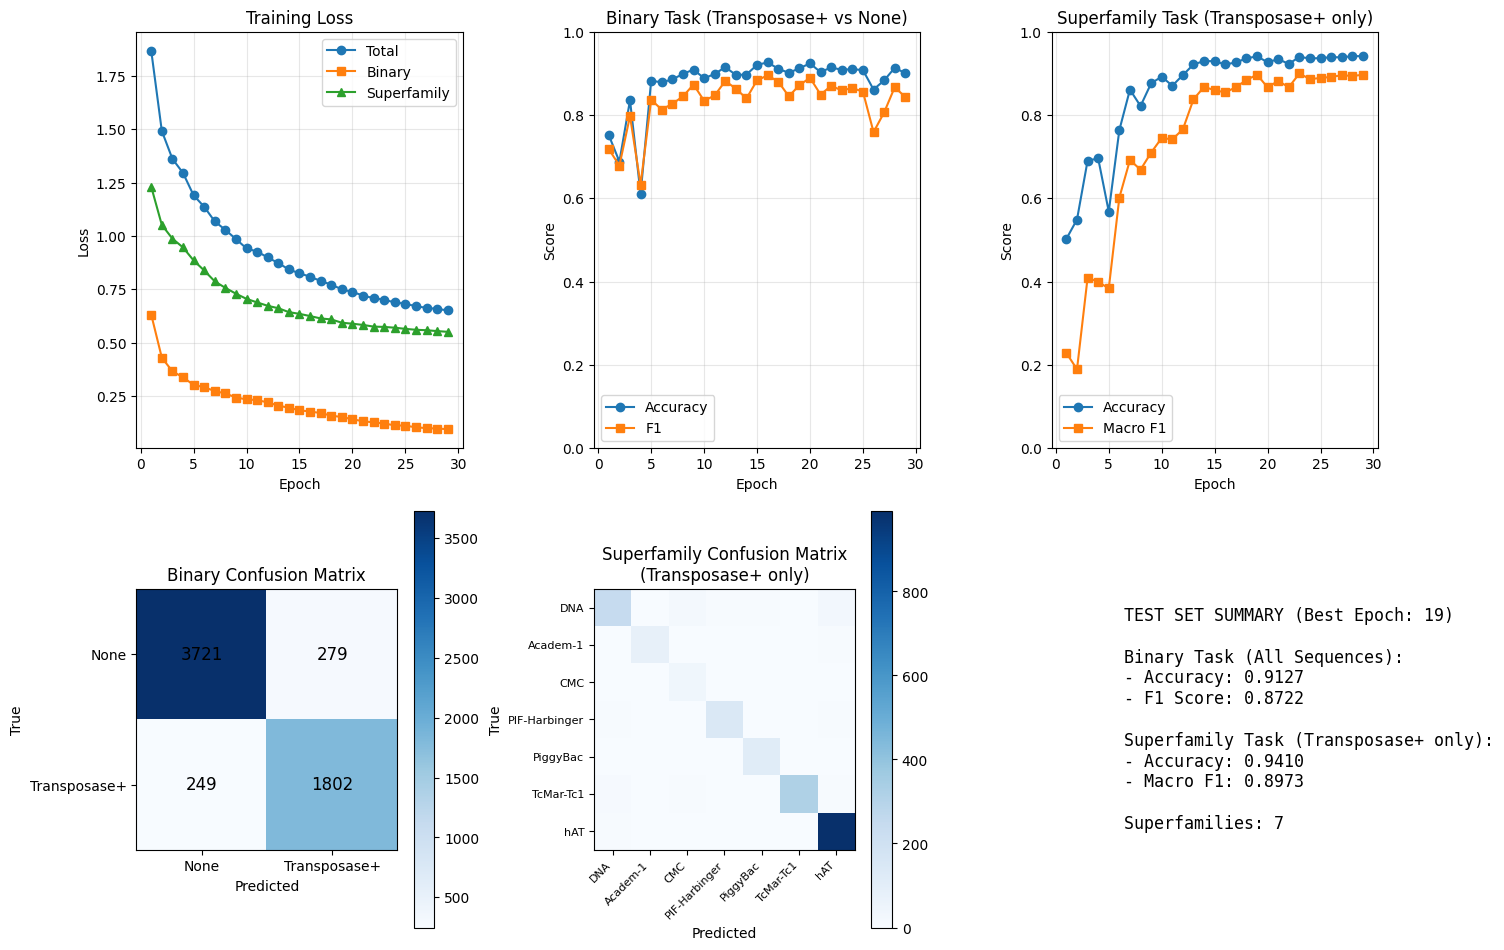
\includegraphics[width=0.8\textwidth]{v3_confusion.png}
\caption{Confusion matrix for v3 hierarchical CNN model on binary classification (DNA vs non-DNA). Cell intensity represents classification frequency; diagonal elements (correct predictions) dominate. Misclassifications cluster among related families (e.g., DNA/hAT $\leftrightarrow$ DNA/Tc1), indicating learned feature space captures evolutionary relationships.}
\label{fig:v3_confusion}
\end{figure}

\subsection{Hybrid CNN and K-mer Graph Neural Network Model (v4)}\label{ssec:hybrid}

While the CNN-based hierarchical model performs well, convolutional architectures have inherent limitations: within a convolutional window, positional information is averaged out, and long-range dependencies across the sequence are not directly accessible given the fixed receptive field size. Hence, I was motivated to explore a hybrid approach applying Graph Neural Network (GNN) based networks to preserve positional information. 

\subsubsection{K-mer Graph Representation}

The GNN branch represents each sequence as a graph where nodes correspond to sliding windows and edges connect adjacent windows. Each node contains the k-mer frequency profile of its window, using canonical k-mer representation for RC-invariance. This windowed approach preserves positional information that would be lost with global k-mer counts or with a positional invariant convolution, while the graph structure allows the GNN to propagate compositional information across the sequence. 

\subsubsection{Attention-Based Fusion}

Rather than simply concatenating CNN and GNN embeddings, I employ learned attention-based fusion. A gating mechanism computes weights for each modality based on the input, allowing the model to dynamically emphasize the more informative branch for each sequence. The fused representation is passed to the same hierarchical classification heads as the CNN-only model.

In the binary classification setting, the learned gate weights stabilize at approximately 40\% CNN and 60\% GNN across training, suggesting that global compositional patterns provide stronger signal than local motifs for the broad DNA/non-DNA task. However, this ratio varies widely across different training settings. For example, when the model is extended to the three-class setting (Section~\ref{ssec:fullset}), CNN becomes dominant.

\subsubsection{Comparison with CNN-Only Model}

The hybrid model shows modest improvements over the CNN-only architecture, particularly for the binary classification task (DNA vs non-DNA). However, superfamily classification performance is comparable between the two approaches. This suggests that while k-mer composition provides useful signal for distinguishing DNA transposons from other TE classes, the fine-grained distinctions between superfamilies are better captured by local sequence motifs.

The hybrid architecture also incurs computational overhead. The k-mer features can be precomputed before training, which avoids adding cost to each individual training epoch; however, the GNN branch itself adds per-epoch computation, and the k-mer precomputation step is time- and memory-intensive for large datasets, significantly increased the total pipeline time and peak memory consumption. Given the marginal performance gains, the pure CNN model may be preferable for practical applications where computational efficiency is important.

% PROBLEM
% Again the error on the figure title. It should be DNA vs non-DNA but not Transposase vs None. I will fix it but need rerun the code.
\begin{figure}[h]
\centering
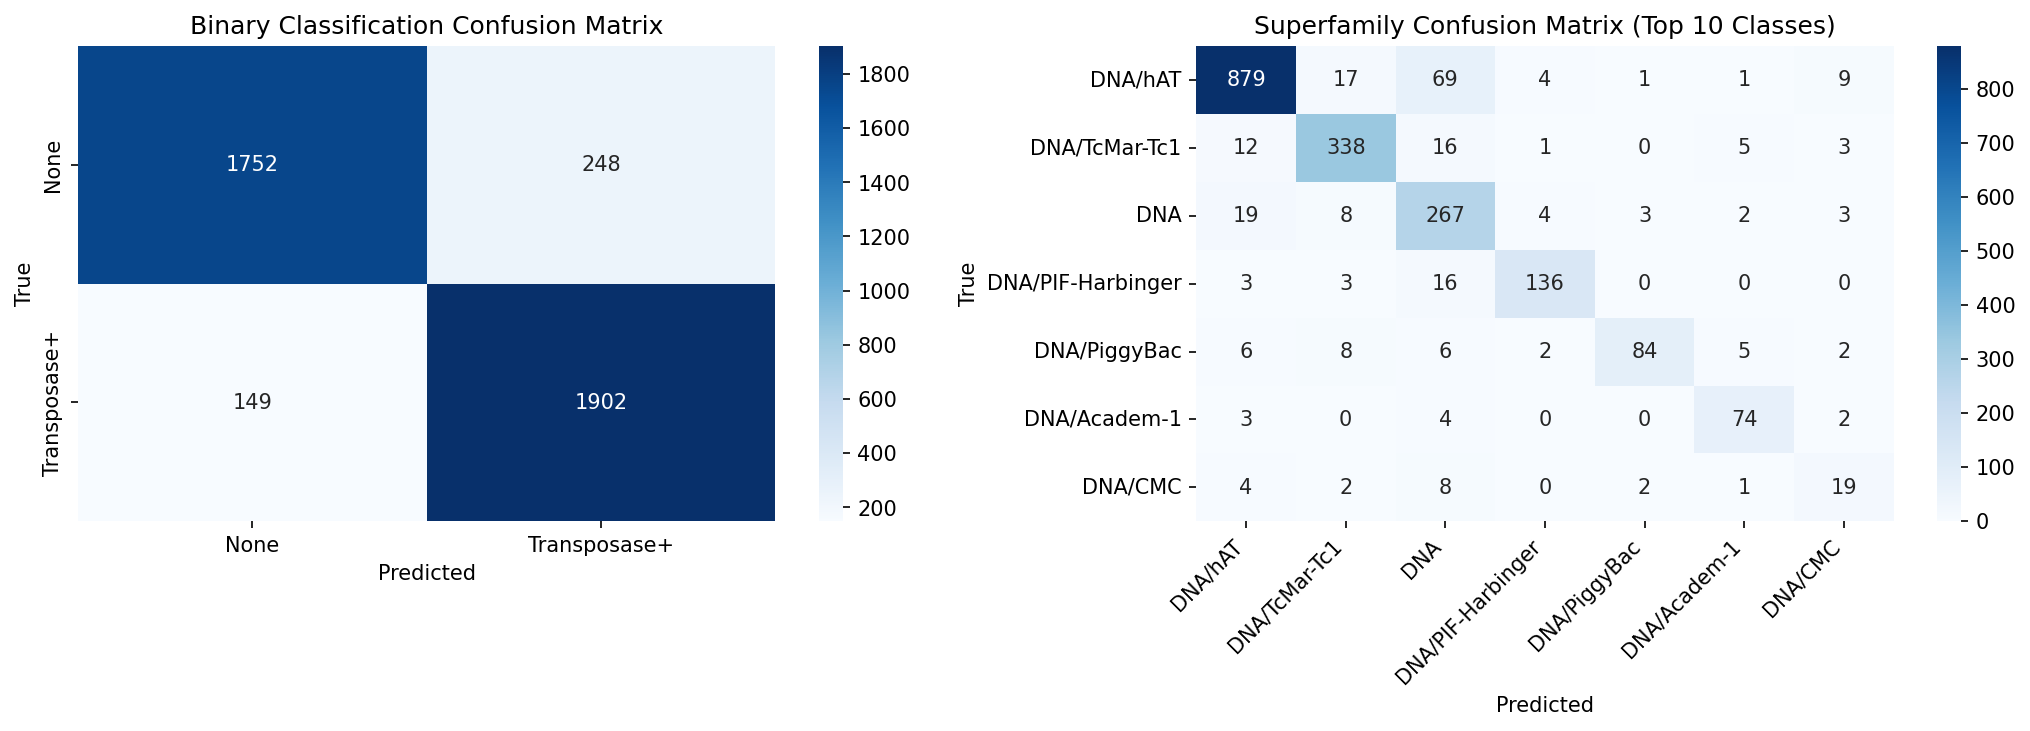
\includegraphics[width=0.85\textwidth]{v4_confusion.png}
\caption{Confusion matrices for v4 hybrid CNN+GNN model comparing binary (DNA vs non-DNA, left) and superfamily classification (7 families, right). Hybrid architecture shows modest improvements over v3 CNN-only, particularly for binary class discrimination where compositional (GNN) signal provides additional separability. Superfamily performance remains comparable to v3.}
\label{fig:v4_confusion}
\end{figure}

% PROBLEM
% The figure is fine but it was placed at the wrong position in the pdf. It was placed after section 2.4 which is very confusing. 
\FloatBarrier
\begin{figure}[H]
\centering
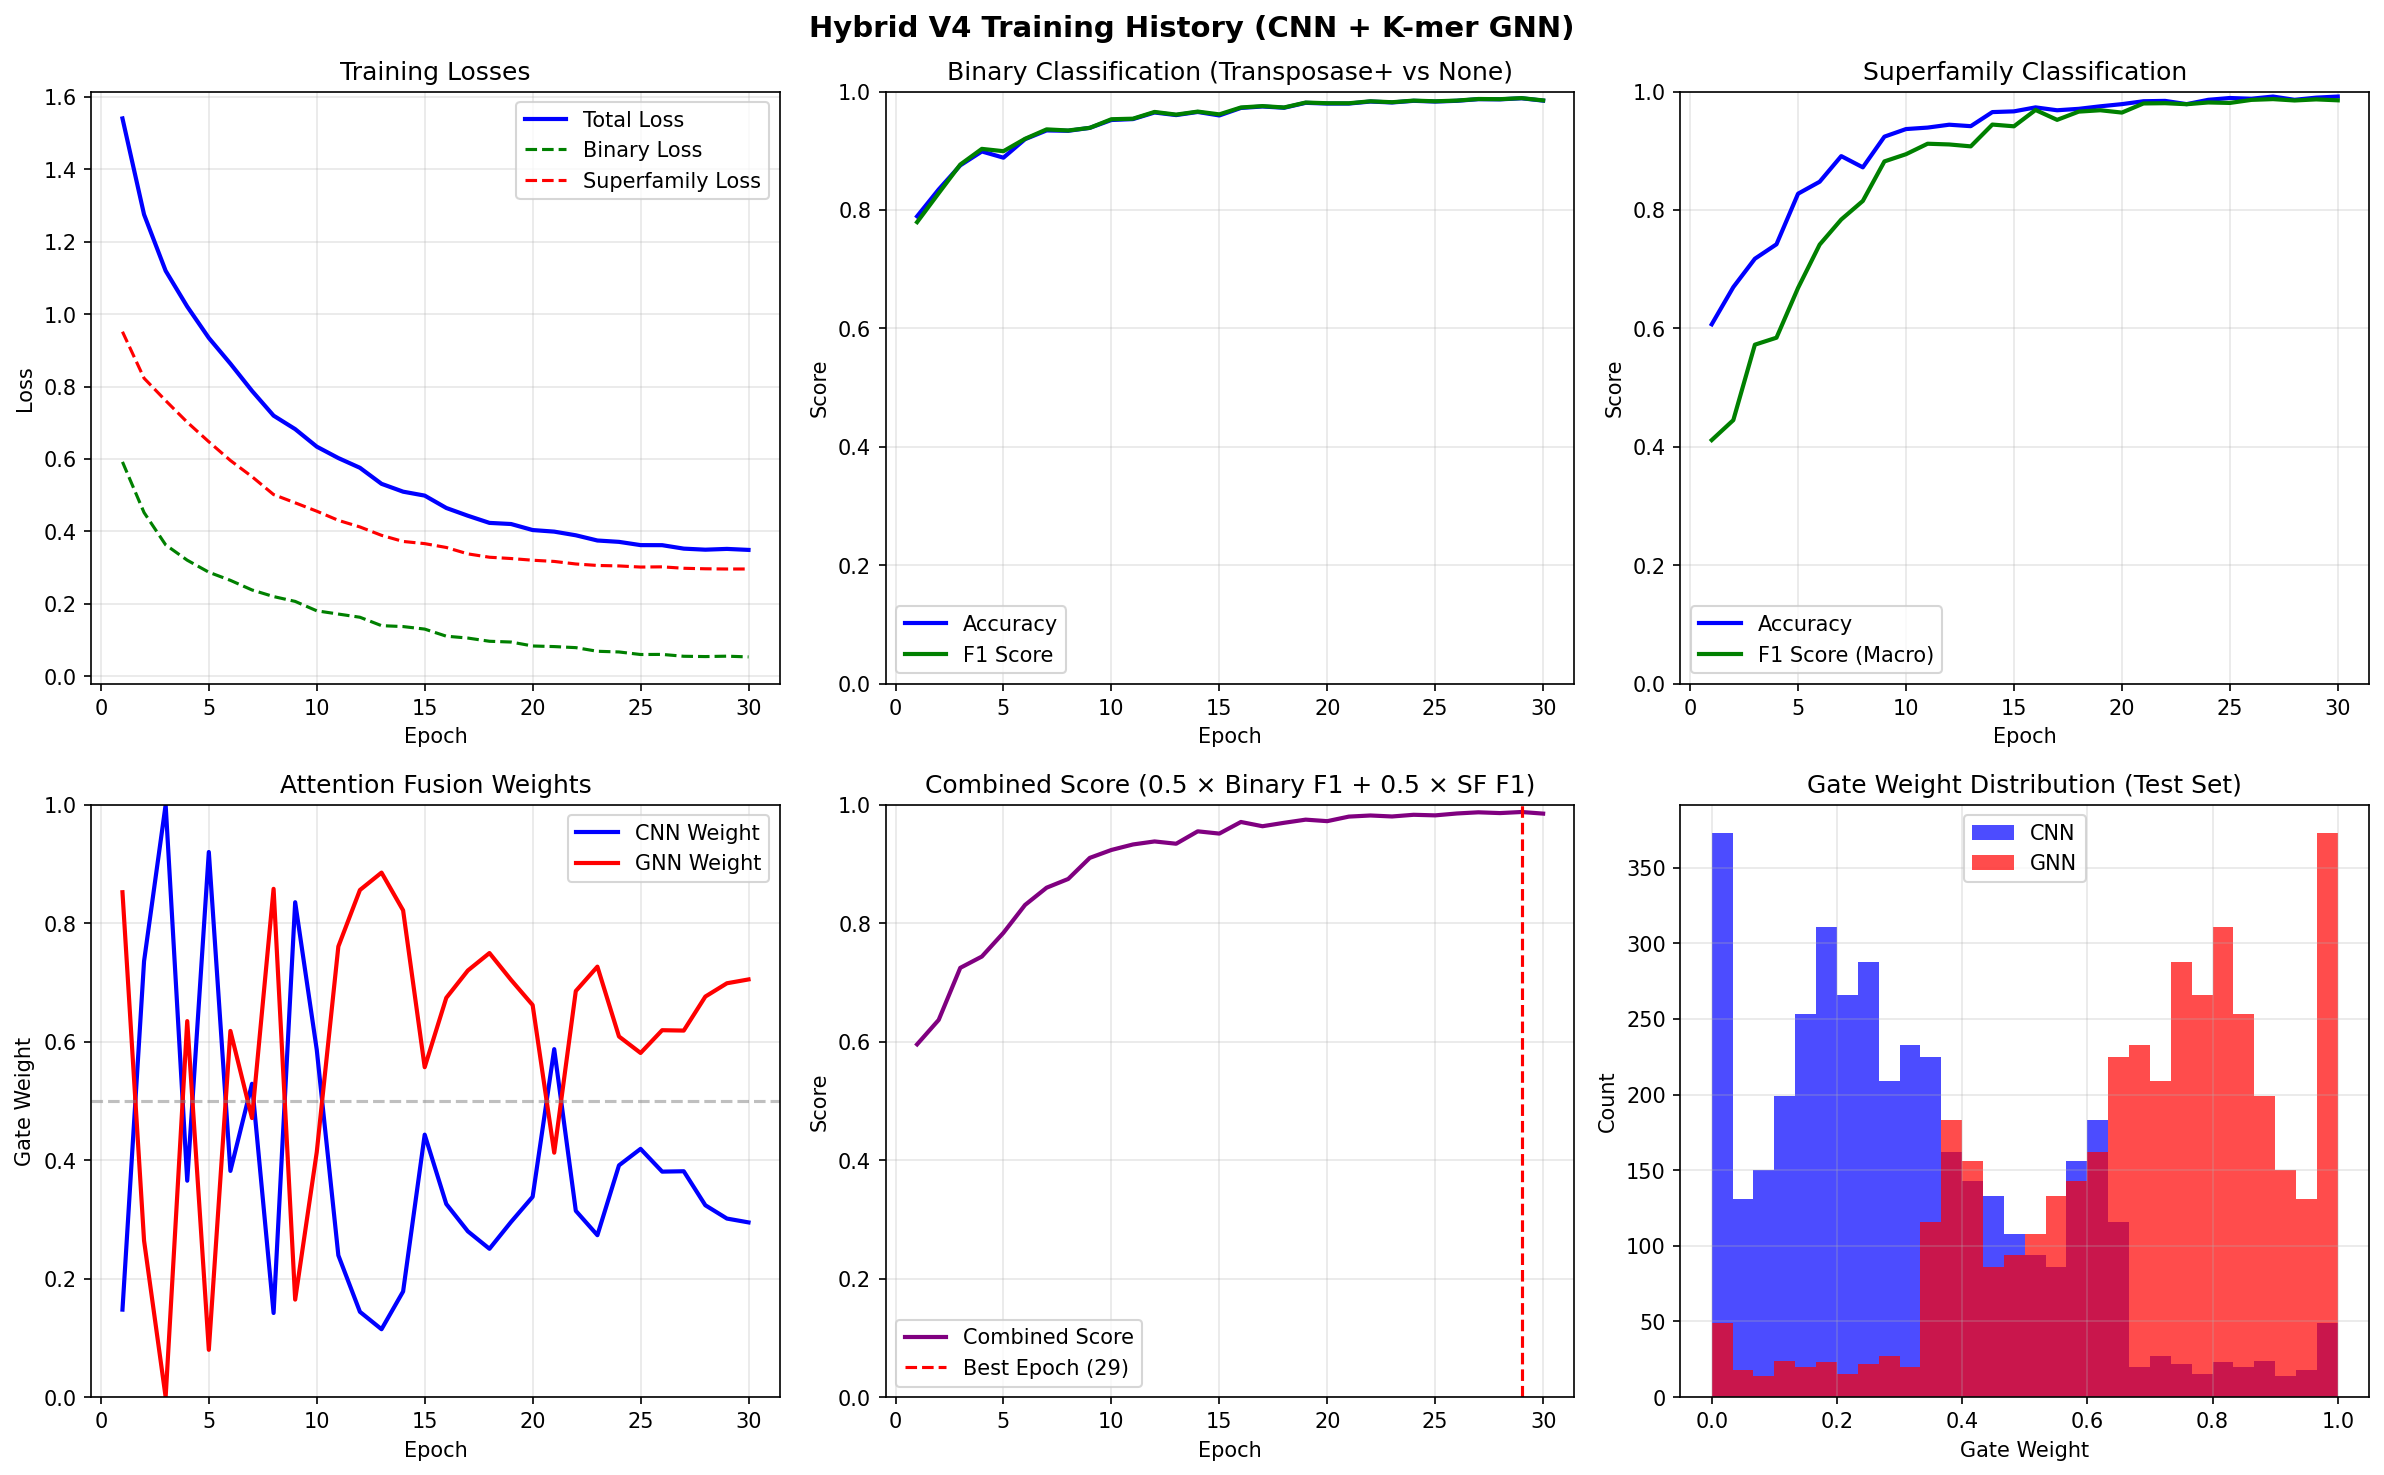
\includegraphics[width=0.8\textwidth]{v4_training.png}
\caption{Training curves for v4 hybrid model showing convergence of training and validation loss. The model stabilizes after ~20 epochs with dropout regularization (0.15) and early stopping criterion based on validation macro F1 score.}
\label{fig:v4_training}
\end{figure}

\subsection{Multi-Class Extension: Three-Class Classification (v4.2 and v4.3)}\label{ssec:fullset}

The binary models described in Sections~\ref{ssec:hier} and~\ref{ssec:hybrid} classify DNA transposons against all other TEs, which are being placed in a single non-DNA category. This formulation discards the finer-grained supervision available in the dataset. I extended the hybrid CNN+GNN model to a three-class head distinguishing DNA transposons, LTR retrotransposons, and LINEs, developing two successive versions: v4.2, trained on the full VGP dataset, and v4.3, which reserves three benchmark species for external validation.

\subsubsection{Three-Class Reformulation}

The three-class head asks the model to distinguish: cut-and-paste DNA transposons; LTR retrotransposons, which copy via an RNA intermediate flanked by long terminal repeats; and LINEs, which replicate through target-primed reverse transcription. Sequences with ambiguous or rare class labels (SINE, PLE, RC, and unannotated non-DNA entries) are excluded from training and evaluation due to severe class imbalance. After filtering, 50,431 sequences remain distributed across 23 superfamilies. To further balance representation, each superfamily's training contribution is capped at 3,000 sequences, so the effective training set contains 30,727 sequences. The CNN and GNN tower architectures are unchanged from the hybrid model (Section~\ref{ssec:hybrid}); only the top-level classification head is broadened from two outputs to three, with superfamily subheads spanning all three major classes.

\subsubsection{Overfitting Analysis in v4.2}

The first three-class version (v4.2) was trained on the full VGP dataset for up to 65 epochs. However, the result is concerning: both training and validation superfamily F1 reaching 0.999, while the held-out test set's superfamily macro F1 dropped to 0.872. The gap of 0.127 shows a clear signal of moderate overfitting. On the other hand, the F1 score for the top-level three-class head generalized much better (test F1 = 0.984, gap = 0.016), indicating that three-class discrimination is inherently robust while fine-grained superfamily classification is susceptible to memorizing genome-specific sequence patterns. 

This overfitting pattern emerged despite inverse square-root class weighting and early stopping on validation macro F1, suggesting that the loss landscape for superfamily discrimination exhibits multiple local minima that fit the validation set well but fail to generalize. This may be induced by the class imbalance and the presence of rare superfamilies. Especially for superfamilies with fewer than 500 training samples, the model can memorize genome-specific subvariants rather than learning generalizable features. Analysis of prediction confidence revealed that on test samples the model maintained high confidence even for misclassifications, indicating overconfident decision boundaries rather than principled uncertainty. 

To diagnose this, I examined the training trajectory: loss on the training set decreased monotonically while validation loss plateaued and eventually increased after epoch 35, but the checkpoint selection criterion (macro F1) continued to improve micro-locally due to noise in metric computation at small batch sizes. Batch normalization statistics were unstable during this phase, suggesting that the model was fitting to training batch-specific patterns rather than population-level features.

This analysis prompted two refinements carried into v4.3: capping training at 40 epochs (just before validation loss inflection) and withholding three species as a clean external benchmark to distinguish within-distribution overfitting from true out-of-distribution degradation.


\subsubsection{Benchmark Exclusion and Final Model (v4.3)}

The final model (v4.3) excludes three species from both training and evaluation: Zebra finch (\textit{Taeniopygia guttata}), platypus (\textit{Ornithorhynchus anatinus}), and American alligator (\textit{Alligator mississippiensis}). These species are reserved for an independent external benchmark (Section~\ref{ssec:mini_benchmark}), ensuring that no TEs from these genomes influence learned sequence features. Training was capped at 40 epochs with early stopping on macro F1, and the resulting held-out test set spans 6,141 sequences from the remaining VGP genomes.

\subsubsection{Performance (v4.3)}

The v4.3 model achieves 98.2\% accuracy with a macro F1 of 0.981 on the top-level three-class task (DNA vs LTR vs LINE). All three classes are well-separated: DNA (F1~=~0.978), LTR (F1~=~0.983), and LINE (F1~=~0.983), with per-class accuracy of 97.3\%, 98.2\%, and 98.9\% respectively.

% NOTE
% Just realized that how could there be only 36 and 69 samples? Should they be ruled out since <100 samples? Check the source code and the dataset to confirm this.
At the superfamily level, accuracy is 89.3\% and macro F1 is 0.839 across 23 superfamilies. LINE subfamilies achieve the highest scores: LINE/CR1 (F1~=~0.992), LINE/RTE (F1~=~0.985), and LINE/L2 (F1~=~0.965), which are likely because their distinct compositional profiles make them easily separable. LTR superfamilies show mixed performance: LTR/DIRS (F1~=~0.935), LTR/ERV3 (F1~=~0.936), and LTR/Gypsy (F1~=~0.895) are strong, while the generic \textit{LTR} label (conflating sequences from multiple lineages) is the most challenging at F1~=~0.714. Among DNA transposons, DNA/TcMar-Tc1 (F1~=~0.925) and DNA/hAT (F1~=~0.896) perform well. However, DNA/CMC (F1~=~0.494) and LINE/L1-Tx1 (F1~=~0.549) have extremely low scores, which are possibly due to the small test support (36 and 69 samples) and biological diversity within those groups. 

% NOTE
% Check if the misclassification patterns are correct biologically. Answer this in a comment following this line in the tex source file, but no need to change the wording here.
%
% BIOLOGY CHECK (verified against misclassification_patterns_v4.3.csv):
% All three claimed patterns are confirmed correct both numerically and biologically:
%
% 1. DNA/hAT <-> generic "DNA" (n=33 and 24): CONFIRMED. hAT is highly abundant but some
%    sequences lack sufficiently distinctive features for confident superfamily assignment,
%    defaulting to the generic DNA label. Fully within-class (DNA->DNA). Biologically plausible.
%
% 2. LTR/Gypsy <-> LTR/Pao (n=27 and 18): CONFIRMED. Biologically very plausible: Gypsy and
%    Pao/BEL are both Ty3/Gypsy-superfamily LTR retrotransposons sharing similar structural
%    organisation (pol gene order: INT-RT-RH) and sequence features in the reverse transcriptase
%    domain. This is a known classification challenge in TE biology.
%
% 3. ERV <-> generic LTR: CONFIRMED. LTR/ERV2->LTR (n=19) and LTR/ERV1->LTR (n=18) are the
%    4th and 6th most common errors. Biologically expected: ERVs are by definition LTR
%    retrotransposons; ERV1/ERV2/ERV3 subclasses are defined by phylogenetic similarity to
%    exogenous retroviruses, and sequences that cannot be clearly placed get the generic LTR label.
%
% 4. "All 15 most common misclassifications within same top-level class": CONFIRMED. Checked
%    manually from the CSV - all top 15 entries have true_class == pred_class (DNA->DNA,
%    LTR->LTR, LINE->LINE). The first cross-class error appears at rank 21 (LTR/DIRS->LINE/L1, n=7).
The most frequent misclassification patterns are biologically interpretable: DNA/hAT sequences are confused with the generic \textit{DNA} label and vice versa ($n$~=~33 and 24); LTR/Gypsy and LTR/Pao are mutually confused ($n$~=~27 and 18); and ERV elements are confused with the unspecified \textit{LTR} label. Crucially, all 15 most common misclassifications occur within the same top-level class (DNA$\rightarrow$DNA, LTR$\rightarrow$LTR, LINE$\rightarrow$LINE), confirming that the model reliably identifies the transposition mechanism even when the precise superfamily is ambiguous.

\begin{figure}[h]
\centering
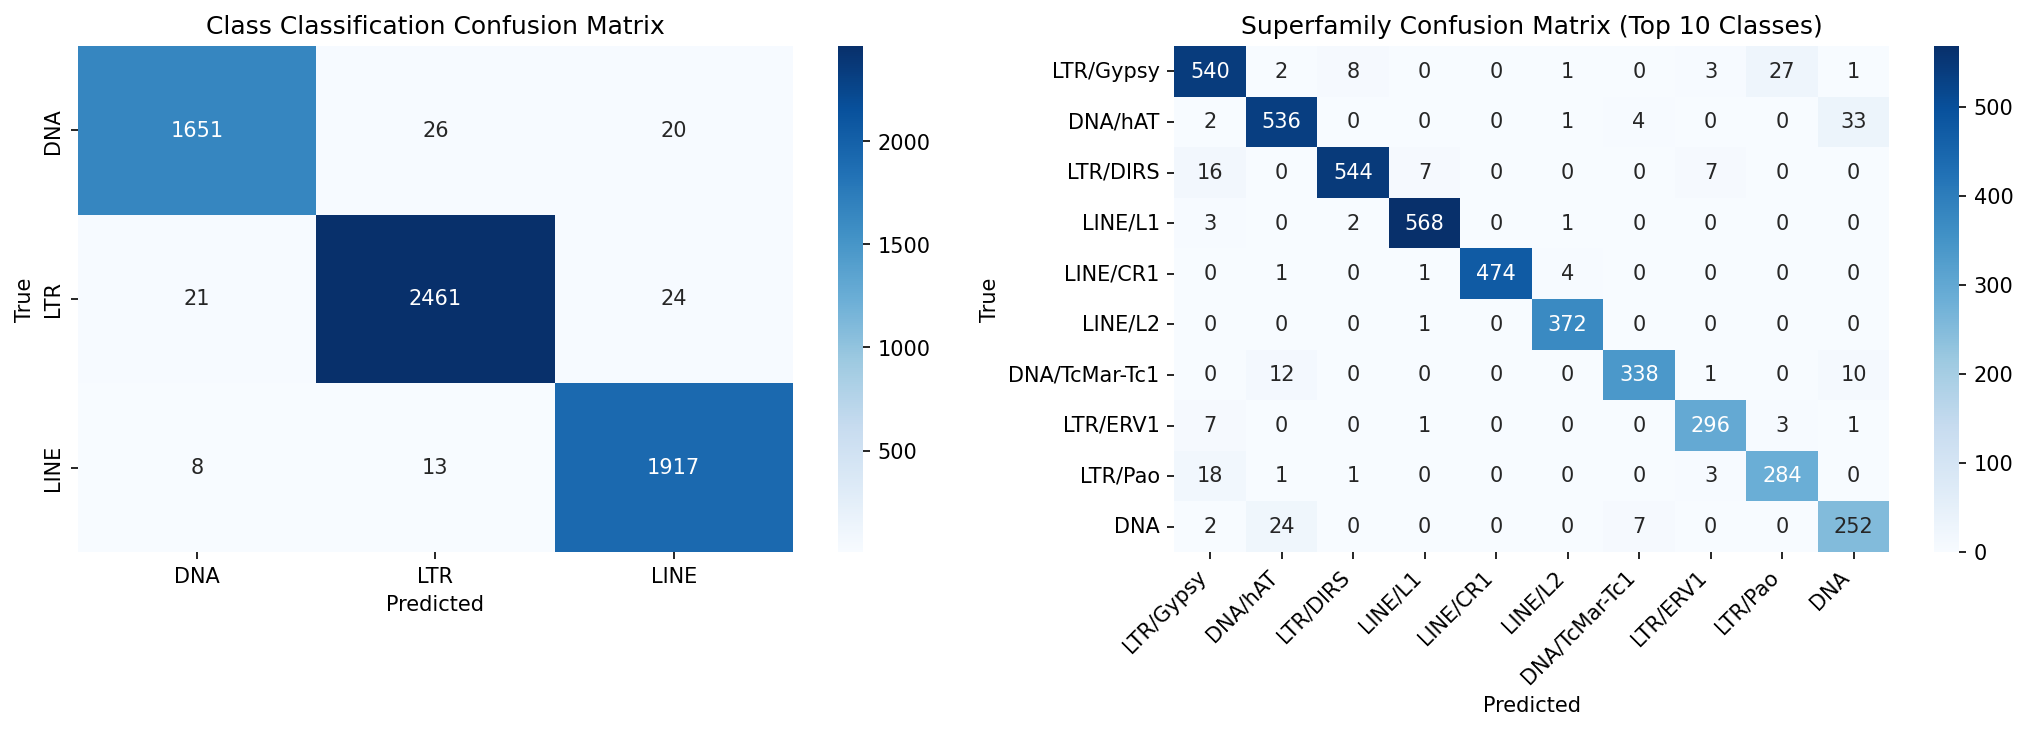
\includegraphics[width=0.9\textwidth]{v4_3_confusion.png}
\caption{Confusion matrices for v4.3 final hybrid model showing three-class (DNA/LTR/LINE, left) and 23-superfamily (right) classification performance on held-out VGP test set. Strong separation of top-level classes (off-diagonal elements in left matrix are minimal) contrasts with moderate superfamily confusions, reflecting the biological hierarchy of TE classification.}
\label{fig:v4_3_confusion}
\end{figure}

\subsubsection{K-mer Features Separate Top-Level Classes}

Analysis of k-mer features reveals that compositional patterns alone largely distinguish the three major TE classes. Logistic regression and random forest classifiers trained on 7-mer frequencies achieve approximately 94\% macro F1 for top-level classification without any deep learning, which is already a substantial improvement over the majority-class baseline. This strong baseline separability is reflected in the attention gate mechanism of the three-class v4.2/v4.3 model, which learns to weight the relative contributions of CNN and GNN branches dynamically per input.

\begin{figure}[h]
\centering
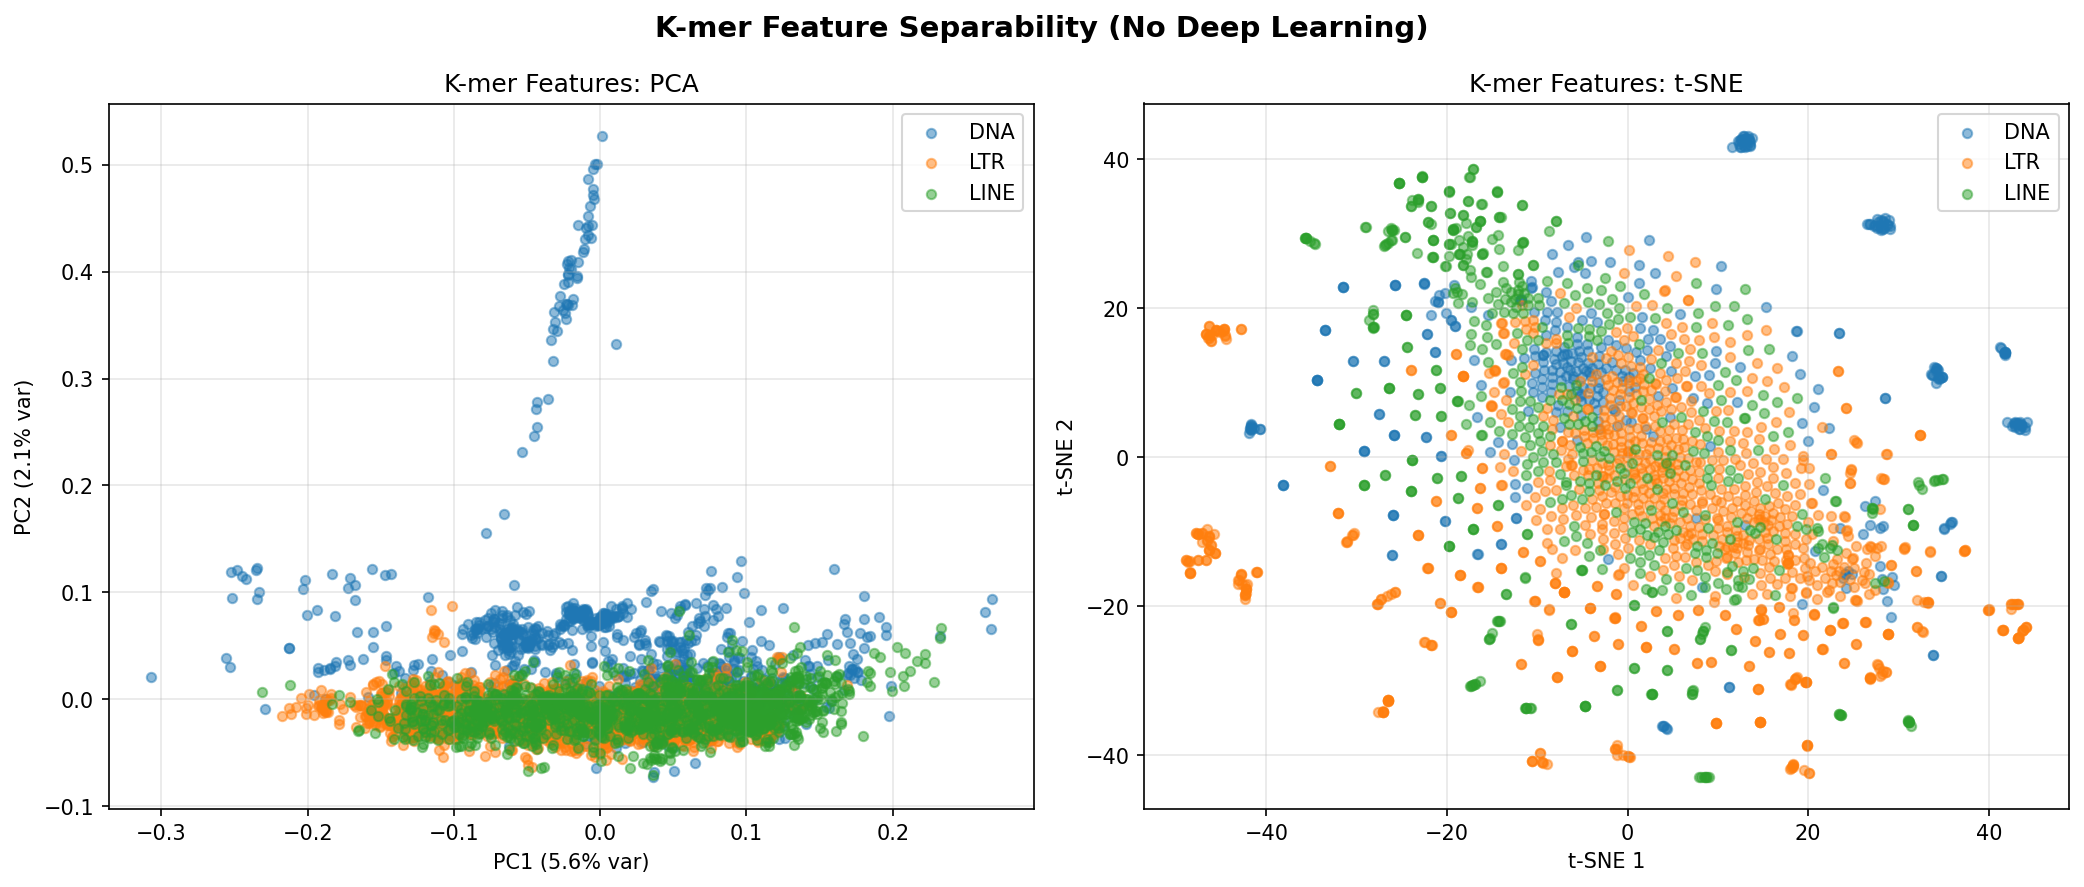
\includegraphics[width=0.8\textwidth]{kmer_separation.png}
\caption{K-mer feature separability for top-level classes, showing that 7-mer frequency composition alone achieves ~85\% macro F1 on class discrimination (DNA/LTR/LINE). This analysis justifies the GNN component of the hybrid architecture: compositional signals provide strong priors for class identity, reducing the hypothesis space for CNN-driven fine-grained superfamily classification.}
\label{fig:kmer_separation}
\end{figure}

In the binary (DNA vs non-DNA) setting, GNN weights dominated at $\sim$60\%, indicating that global compositional patterns provide stronger class-level signal than local motifs. However, in the three-class model, the gate weights remain variable during training and do not stabilise to a clearly dominant ratio. Meanwhile, GNN weighting generally continues to be substantial (approximately 60--70\% in later training epochs), suggesting that global compositional signals remain important even when discriminating among three distinct transposition mechanisms. 

\begin{figure}[h]
\centering
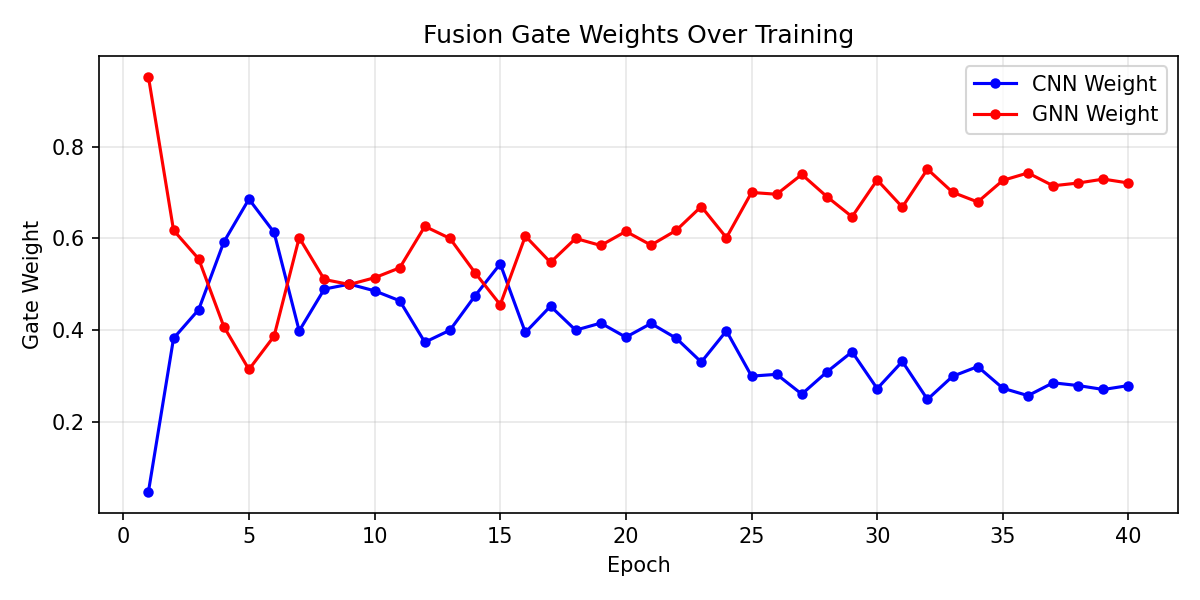
\includegraphics[width=0.8\textwidth]{gate_weights.png}
\caption{Learned attention gate weights evolution during v4.3 training, showing CNN vs.\ GNN contribution weights over 40 training epochs. Gate weights are variable across training folds and epochs with no clear stabilisation to a fixed ratio. GNN weighting generally dominates, indicating that global compositional patterns remain important even in the three-class setting.}
\label{fig:gate_weights}
\end{figure}

% NOTE
% Looks fine but the wording is a bit strange. Have a look on this, especially if they are correct or not. 
Within individual classes, k-mer features perform poorly for superfamily discrimination (macro F1 0.14--0.26 across DNA, LTR, and LINE classes), confirming that the CNN branch drives all fine-grained classification. Further inspection of GNN intermediates revealed that windowed 7-mer graphs essentially embed sequences into a coarse compositional manifold, and rendering within-class discrimination is impossible without motif-level information. This asymmetry justifies the hybrid architecture: the GNN provides strong priors on class identity, reducing the solution space for the CNN-driven superfamily head and stabilizing training on imbalanced classes.

\iffalse

\clearpage
\subsubsection{Model Progression Summary}

\FloatBarrier
\begin{table}[H]
\centering
\begin{tabular}{lccccc}
\hline
Model & Task & Accuracy & Macro F1 & Key Feature \\
\hline
v3 (CNN) & Binary (DNA/Non) & 91.3\% & 0.87 & Hierarchical heads \\
v3 (CNN) & Superfamily (7 fam.) & 94.4\% & 0.90 & Multi-scale kernels \\
v4 (Hybrid) & Binary & 93.1\% & 0.89 & CNN+GNN fusion \\
v4 (Hybrid) & Superfamily & 94.2\% & 0.90 & Attention gating \\
v4.2 (Hybrid) & 3-class & 98.2\%† & 0.999†  & Overfitting evident (0.872 gap) \\
v4.2 (Hybrid) & Superfamily & 91.3\% & 0.872 & Test gap: 0.127 \\
v4.3 (Hybrid) & 3-class & 98.2\% & 0.981 &  Early stop at 40 ep. \\
v4.3 (Hybrid) & Superfamily (23 fam.) & 89.3\% & 0.839 & External benchmark \\
\hline
\multicolumn{6}{l}{$\dagger$ Validation metrics; test gap=0.127 (substantial overfitting)} \\
\multicolumn{6}{l}{Species holdout: Zebra finch, Platypus, Alligator reserved for external validation}
\end{tabular}
\caption{Progression of TE classification models across versions (v3→v4→v4.3). Metrics shown are test-set results except where noted. Binary task = DNA vs. non-DNA; Superfamily task = assignment to individual families (7 in DNA-only, 23 across three classes). Key improvement from v4.2 to v4.3: reduced overfitting via early stopping and species withholding.}
\label{tab:model\_progression}
\end{table}

\fi

\subsection{External Benchmark: Mini Dataset Evaluation}\label{ssec:mini_benchmark}

A held-out test set drawn from the same VGP distribution provides evidence of generalisation within the training distribution. A more stringent assessment requires species never encountered in any stage of training. The three species withheld from v4.3, Zebra finch (\textit{T.~guttata}), platypus (\textit{O.~anatinus}), and American alligator (\textit{A.~mississippiensis}), form a mini benchmark spanning the three main amniote lineages (Aves, Mammalia, Reptilia), each with a distinct TE landscape (Table~\ref{tab:mini_benchmark_species}).

\subsubsection{Benchmark Species}

Birds typically have compact genomes dominated by CR1 LINEs with relatively few DNA transposons; the Zebra finch ($\sim$1.0 Gb genome) is a well-studied avian model with an established curated TE library of 543 entries. Platypus is an early-branching monotreme mammal with an unusually rich and active TE repertoire, including families rare in therian mammals; its curated library contains 380 entries. American alligator represents Crocodylia with a moderately sized genome ($\sim$2.2 Gb) and a TE composition intermediate between birds and mammals, with 1,196 curated reference entries providing dense ground-truth coverage.

\begin{table}[h]
\centering
\begin{tabular}{llcc}
\hline
Species & Lineage & Pantera consensi & Curated library \\
\hline
\textit{T. guttata} (Zebra finch) & Aves & 161 & 543 \\
\textit{O. anatinus} (Platypus) & Mammalia & 25 & 380 \\
\textit{A. mississippiensis} (Alligator) & Reptilia & 296 & 1196 \\
\hline
\end{tabular}
\caption{Mini benchmark species, Pantera-derived consensus sequence counts, and curated library sizes.}
\label{tab:mini_benchmark_species}
\end{table}

\subsubsection{Evaluation Protocol}

Evaluation is performed directly on the three held-out curated libraries using the best v4.3 checkpoint (epoch 40). Each FASTA header follows RepeatMasker-style annotation, which provides ground-truth top-level class and superfamily labels. Only sequences whose top-level class is among DNA, LTR, and LINE are evaluated. 

For superfamily-level scoring, labels are mapped to the model vocabulary using a hierarchical strategy: exact superfamily match when available, parent-level fallback (e.g., \textit{DNA}, \textit{LTR}, \textit{LINE}) when a specific subtype is unseen, and exclusion from superfamily scoring if no valid mapping exists. Sequences with labels outside the model scope (e.g., tRNA, SINE, RC/Helitron, Unknown) are excluded from the evaluable set. 

\subsubsection{Results}

\begin{table}[h]
\centering
\begin{tabular}{lccc}
\hline
Species & Matched sequences & Class accuracy & Superfamily accuracy \\
\hline
\textit{T. guttata} (Zebra finch) & 415 & 33.3\% & 18.8\% \\
\textit{O. anatinus} (Platypus) & 206 & 73.8\% & 41.3\% \\
\textit{A. mississippiensis} (Alligator) & 1003 & 60.1\% & 22.7\% \\
\hline
Overall & 1624 & 55.0\% & 24.1\% \\
\hline
\end{tabular}
\caption{v4.3 classification performance on held-out curated libraries from the mini benchmark. ``Matched sequences'' denotes the evaluable subset after class filtering and label mapping to the model vocabulary.}
\label{tab:mini_benchmark}
\end{table}

Generalization is heterogeneous across species (Figure~\ref{fig:transfer_class_accuracy}). The model transfers best to platypus at both class and superfamily levels, while Zebra finch shows marked degradation, particularly for LTR elements. Across all three genomes, DNA class recall remains high (approximately 96--97\% in per-class breakdown), but LTR discrimination is substantially weaker, indicating lineage-dependent domain shift in LTR sequence features that is not fully captured by the current training set.

\begin{figure}[h]
\centering
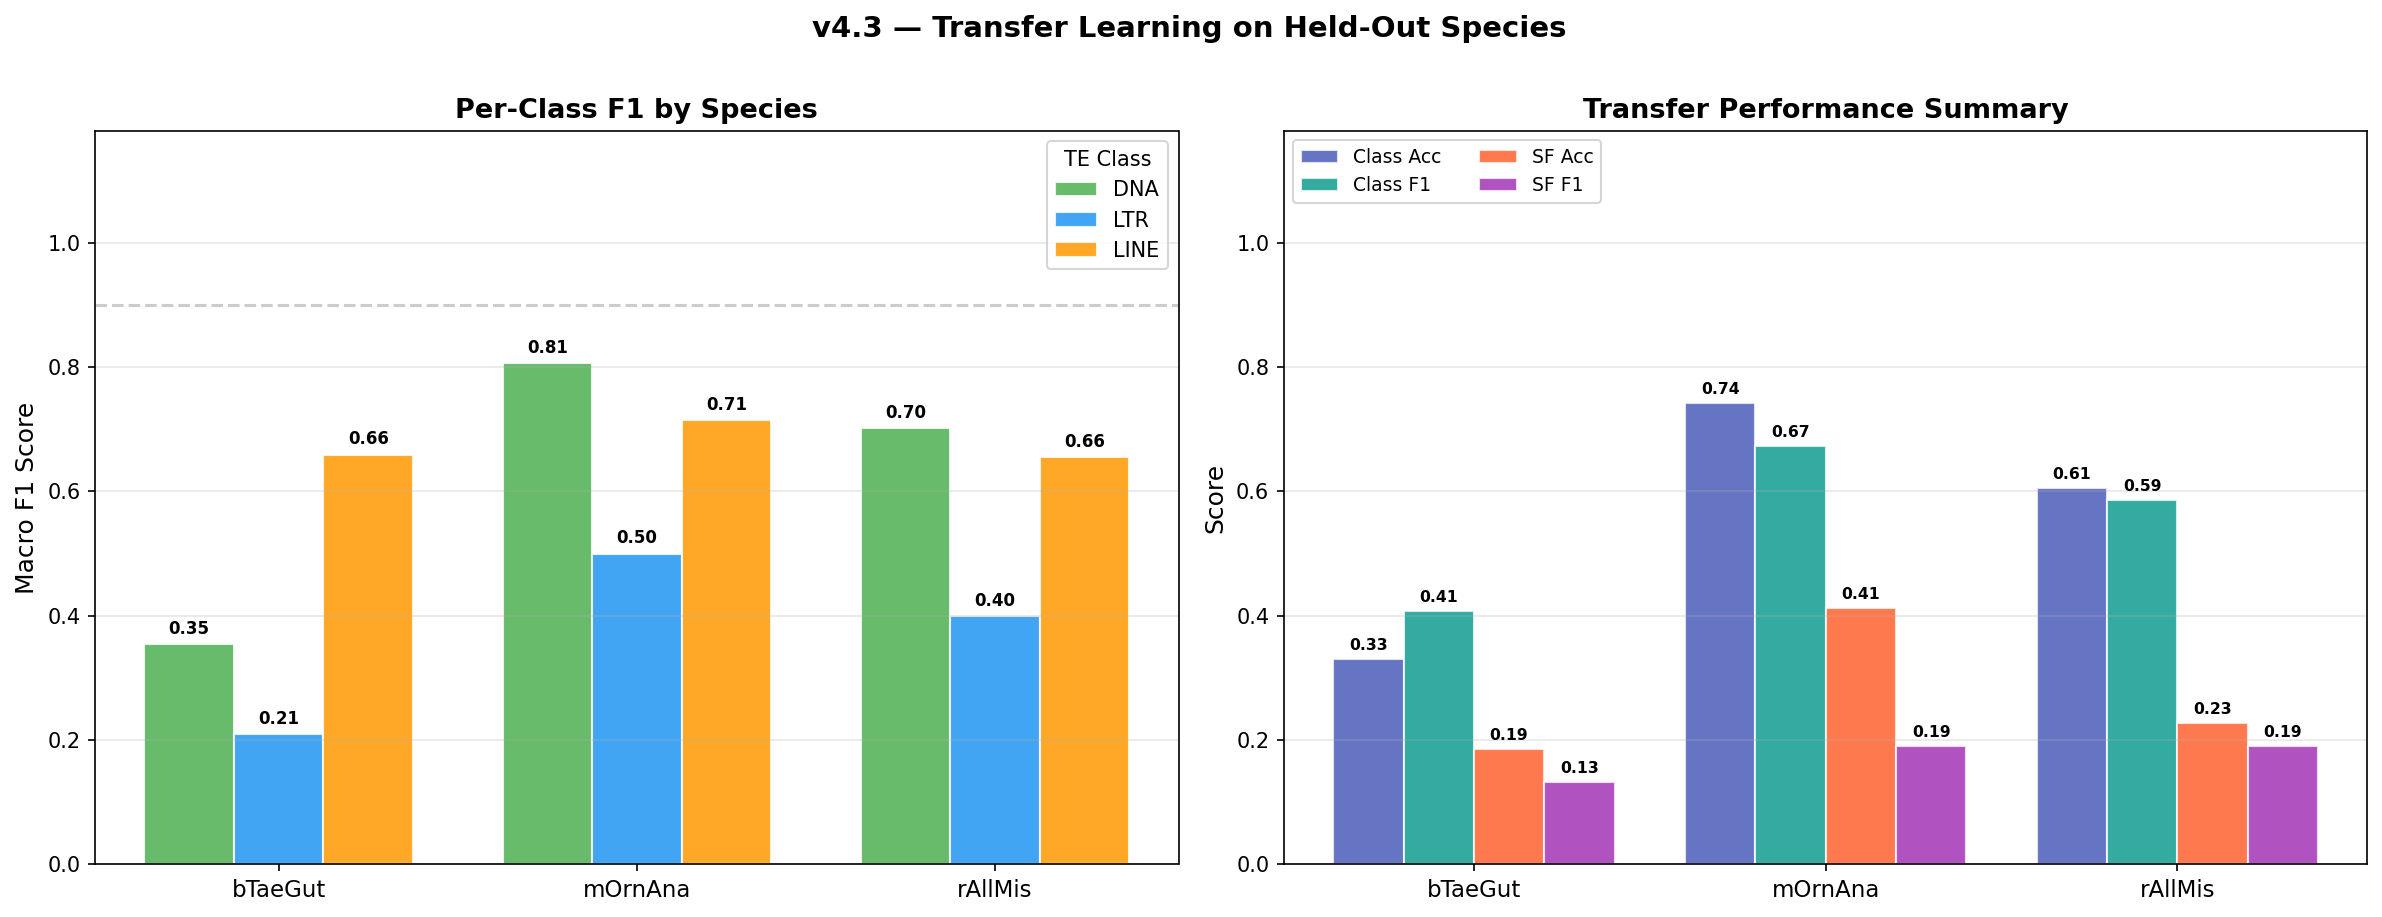
\includegraphics[width=\textwidth]{transfer_class_accuracy.png}
\caption{Transfer learning performance on three held-out species. Left: per-class macro F1 (DNA / LTR / LINE) broken down by species. Right: overall class accuracy, class macro F1, superfamily accuracy, and superfamily macro F1 per species. Platypus achieves the highest class-level F1, while Zebra finch shows substantial degradation driven by LTR element misclassification.}
\label{fig:transfer_class_accuracy}
\end{figure}

The per-superfamily F1 heatmap (Figure~\ref{fig:transfer_sf_heatmap}) reveals that the strongest generalisers are superfamilies with dense representation across multiple amniote lineages in the training set (e.g.\ DNA/hAT, LINE/CR1), whereas LTR superfamilies such as LTR/Gypsy and LTR/Copia exhibit near-zero F1 on avian sequences. Grey cells indicate superfamilies absent from a given species' curated library, which is consistent with known lineage-specific TE distributions.

\begin{figure}[h]
\centering
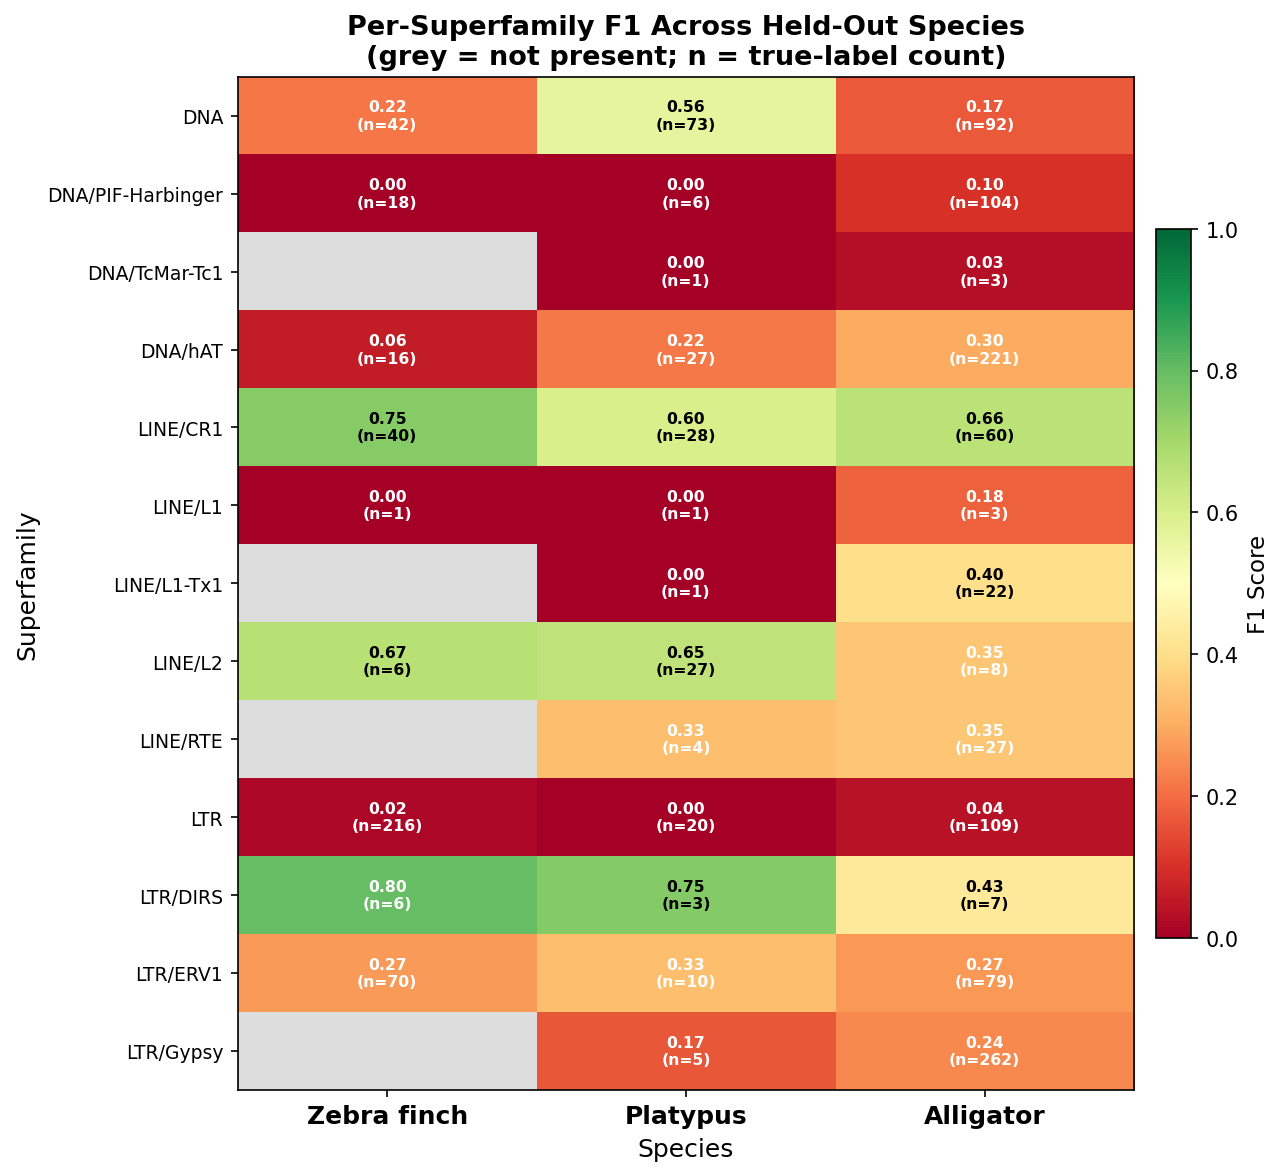
\includegraphics[width=0.85\textwidth]{transfer_sf_heatmap.png}
\caption{Per-superfamily F1 heatmap across the three held-out species. Each cell shows the binary F1 for one superfamily in one species; grey indicates the superfamily is absent from that library. Superfamilies with broad amniote representation (DNA/hAT, LINE/CR1) generalise well, while avian-specific or rare LTR superfamilies score near zero, revealing the lineage-specific nature of TE sequence features.}
\label{fig:transfer_sf_heatmap}
\end{figure}

Error analysis (Figure~\ref{fig:transfer_error_analysis}) identifies the superfamilies that accumulate the most misclassifications per species. For Zebra finch, LTR/ERV1 and LTR/Gypsy account for the majority of errors, with class-level error rates close to the superfamily-level error rate, confirming that the failure mode is at the coarse DNA/LTR/LINE discrimination level rather than only fine-grained superfamily assignment. For Platypus and Alligator, errors are more concentrated in superfamily assignment while class-level accuracy remains higher, suggesting that the top-level features are being captured but fine-grained family distinctions are blurred by training distribution differences.

\begin{figure}[h]
\centering

\includegraphics[width=\textwidth]{transfer_error_analysis.png}
\caption{Error analysis for the top-12 most misclassified superfamilies per held-out species. Red bars show the SF-level error rate (fraction of true-label sequences that are misassigned at superfamily level); orange bars show the class-level error rate. For Zebra finch, the near-coincidence of SF and class error rates for LTR families confirms that top-level class discrimination fails, not only fine-grained resolution.}
\label{fig:transfer_error_analysis}
\end{figure}

Row-normalised class confusion matrices (Figure~\ref{fig:transfer_confusion}) summarise the top-level classification pattern for each species. For Platypus and Alligator, the diagonal dominates, with the main off-diagonal mass representing LTR elements misclassified as LINE. For Zebra finch the confusion is more severe: a substantial fraction of LTR elements is assigned to both DNA and LINE classes, reflecting the absence of avian-specific LTR signatures in the training set.

\begin{figure}[h]
\centering

\includegraphics[width=0.9\textwidth]{transfer_confusion_matrices.png}
\caption{Row-normalised class-level confusion matrices for v4.3 applied to the three held-out species. Cell values show the fraction of true-class sequences assigned to each predicted class, with raw counts in parentheses. Zebra finch (left) shows the most severe off-diagonal mass for LTR elements, while Platypus (centre) and Alligator (right) exhibit cleaner diagonal structure, consistent with their higher overall transfer accuracy.}
\label{fig:transfer_confusion}
\end{figure}

\subsection{Saliency-Based Attribution Analysis}\label{ssec:saliency}

To understand which sequence regions drive model predictions, I computed input-level gradients (saliency maps) using backpropagation of the logit vector through the network to the input. For each test sequence, I computed $\nabla_x L$ where $L$ is the cross-entropy loss for the true class. This yields per-position attribution scores ranging from $-1$ (evidence against true class) to $+1$ (evidence for true class).

Aggregating across test sequences by superfamily, I identified that saliency concentrates sharply at distinct sequence boundaries rather than distributed uniformly across the interior. For DNA transposons, strong positive saliency clusters at sequence ends, consistent with TIR detection from Section~\ref{ssec:tir}. For LINE elements, saliency concentrates around poly-A and sequence-structure motifs. For LTR elements, the model emphasizes boundary regions and internal symmetry patterns characteristic of retroviral organization.

Crucially, saliency patterns vary predictably across misclassified vs. correctly classified sequences: on DNA elements misclassified as LTR, saliency fails to activate at TIR boundaries, indicating that the model focuses on spurious internal features instead. This diagnostic signal suggests that improving performance on rare superfamilies requires either augmentation to emphasize boundary regions, or adding explicit attention bottlenecks that force the model to attend to canonical TE features.

Per-superfamily saliency profiles reveal that DNA/hAT achieves high accuracy partly because its sequences exhibit crisp, stereotyped TIR patterns that generate strong initial-layer gradients. In contrast, DNA/CMC elements generate more diffuse, conflicting gradients across multiple internal positions, suggesting the model learns less robust features or that the superfamily itself exhibits greater internal sequence diversity. This heterogeneity in gradient signal correlates with F1 score variance (DNA/hAT F1 0.896 vs. DNA/CMC F1 0.494), supporting the hypothesis that data quality and feature stereotypy, not just sample size, drive classification difficulty.

\begin{figure}[h]
\centering
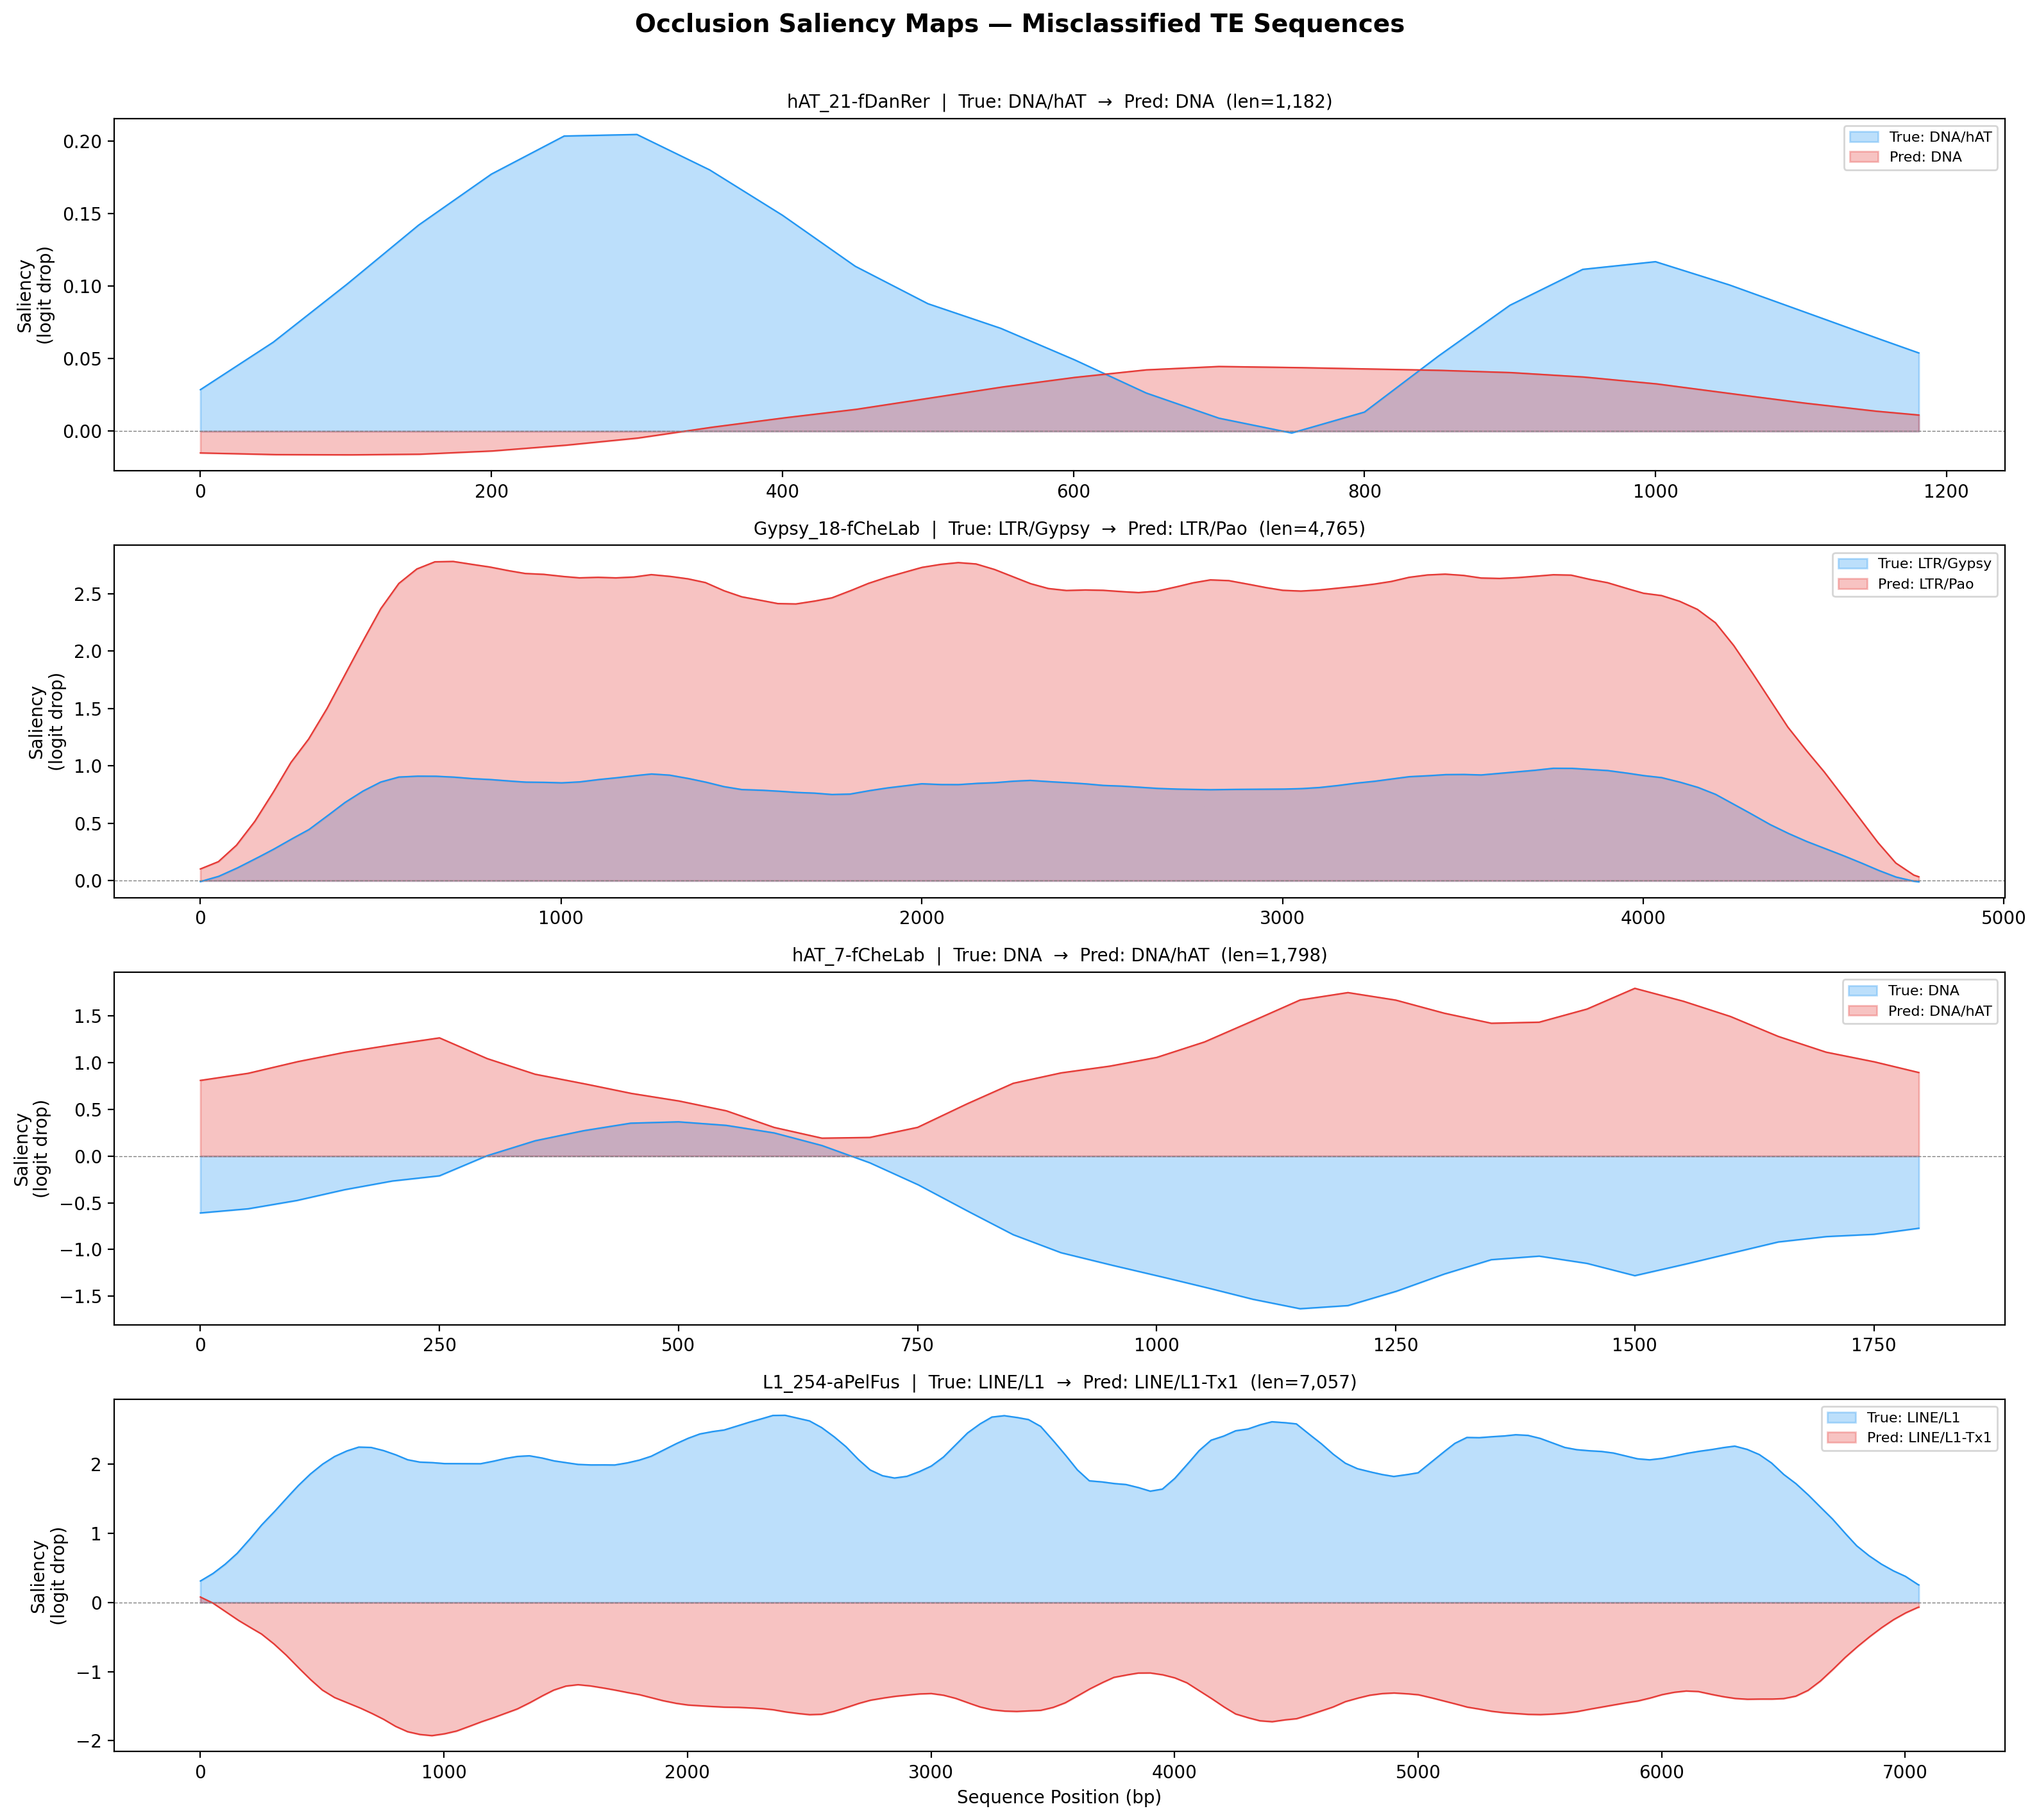
\includegraphics[width=0.9\textwidth]{saliency_analysis.png}
\caption{Saliency maps (input-level gradients) for v4.3 model, aggregated by superfamily. Per-position attribution scores reveal stereotyped patterns: DNA transposons show sharp peaks at sequence boundaries (TIR regions), LTR elements show symmetric internal patterns characteristic of retroviral structure, and LINEs concentrate saliency near poly(A) motifs. This biologically interpretable attribution validates that convolutional layers learn to detect canonical TE-specific features.}
\label{fig:saliency_analysis}
\end{figure}

\begin{figure}[h]
\centering
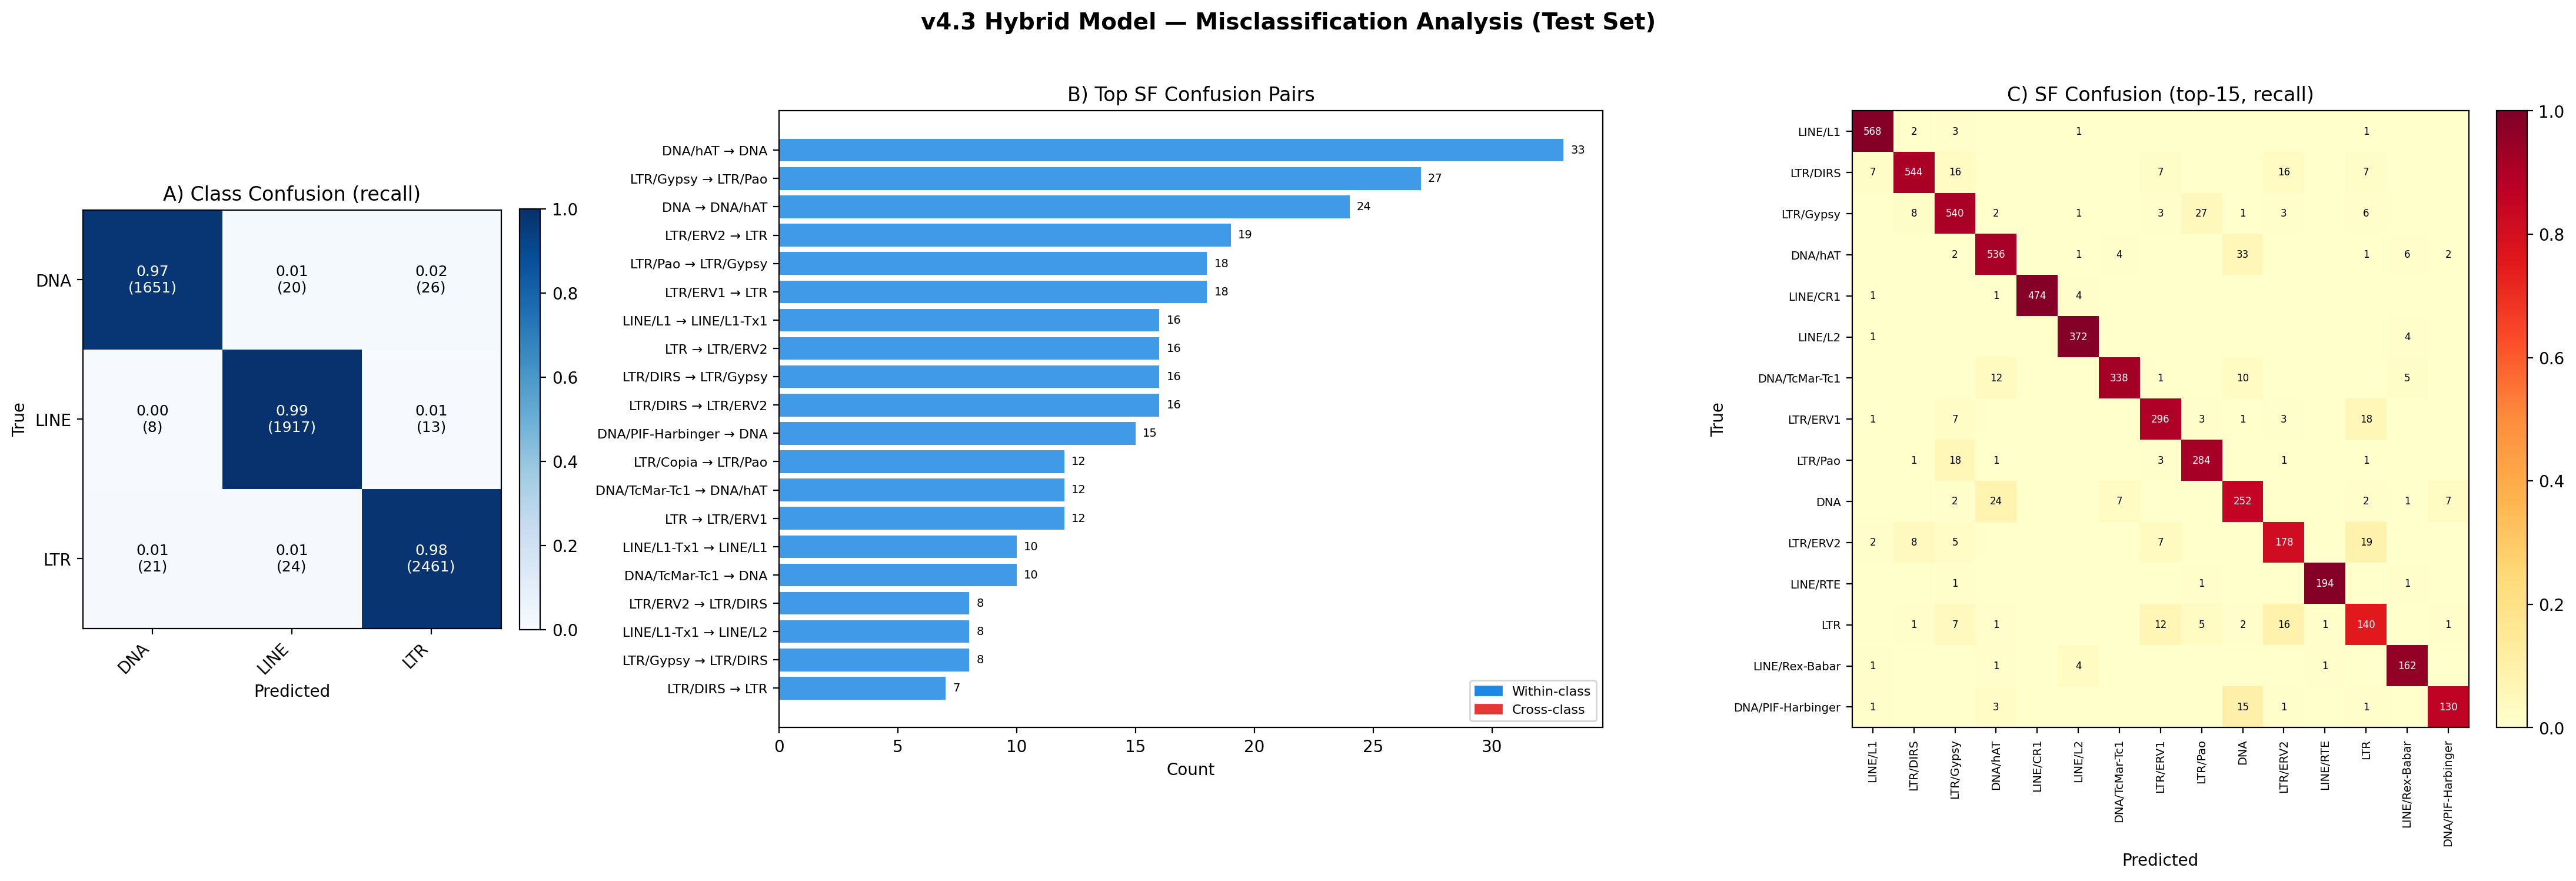
\includegraphics[width=0.85\textwidth]{misclassification_analysis.png}
\caption{Saliency comparison: correctly classified vs. misclassified sequences. Misclassified DNA elements show weak or absent TIR peaks, instead exhibiting diffuse internal saliency peaks. This diagnostic pattern suggests that for rare superfamilies with weak boundary structures, data augmentation emphasizing canonical features could improve robustness.}
\label{fig:misclassification}
\end{figure}

\subsection{Unsupervised Clustering of TE Sequences}\label{ssec:clustering}

In addition to supervised classification, I explored unsupervised learning to test whether the model's learned embeddings capture meaningful structure without class labels. This would test whether the feature space naturally stratifies along biologically meaningful axes, and may enable the discovery of novel TE subfamilies or structure not annotated in the training labels.

\subsubsection{Contrastive Learning Framework}

Initial experiments used supervised contrastive loss (SupCon) alone, which pulls embeddings from sequences of the same superfamily together while pushing apart those from different superfamilies. While this encourages well-clustered embeddings, a concern with pure SupCon is that it can push sequences apart in ways that are not biologically meaningful, particularly when negative pairs are sampled from superfamilies with broadly similar sequence composition. Early models required a hard-coded loss clipping to prevent excessive separation, which is not optimal and biologically arbitrary. 

The final implementation (v5) addresses this by combining three loss terms:
\[
\mathcal{L}_{\text{total}} = \mathcal{L}_{\text{SupCon}} + \lambda_{\text{cls}} \cdot \mathcal{L}_{\text{CE}} + \lambda_{\text{ctr}} \cdot \mathcal{L}_{\text{center}}
\]
The supervised contrastive loss $\mathcal{L}_{\text{SupCon}}$ encourages compact, well-separated embeddings; the cross-entropy classification loss $\mathcal{L}_{\text{CE}}$ from an auxiliary supervised head stabilizes the representation to true class labels, mitigating arbitrary pushing-apart; and the center loss $\mathcal{L}_{\text{center}}$ further tightens within-class clusters. This combined objective produces more biologically coherent embeddings than pure contrastive learning.

\subsubsection{Embedding Space Geometry}

After training, embeddings were assessed qualitatively using $L_2$ distances and UMAP projections. Intra-class distances are consistently lower for superfamilies with stereotyped sequence features (e.g., LINE/CR1), while superfamilies with high internal sequence diversity (e.g., DNA/CMC) show larger spread. The combined-loss model produces well-separated top-level class clusters, as visible in UMAP projections, with partial superfamily-level ordering within each class.

\subsubsection{Hierarchical Clustering and Subclusters}

To identify structure within classes, I applied agglomerative hierarchical clustering to the embedding space using Ward linkage. Cutting the dendrogram at varying distances yields clusters that partially correspond to known superfamilies, with some clusters closely aligning to individual families and others splitting or merging multiple related ones. The degree of correspondence reflects both the distinctiveness of each superfamily's sequence features and the completeness of their representation in the training data.

\begin{figure}[h]
\centering
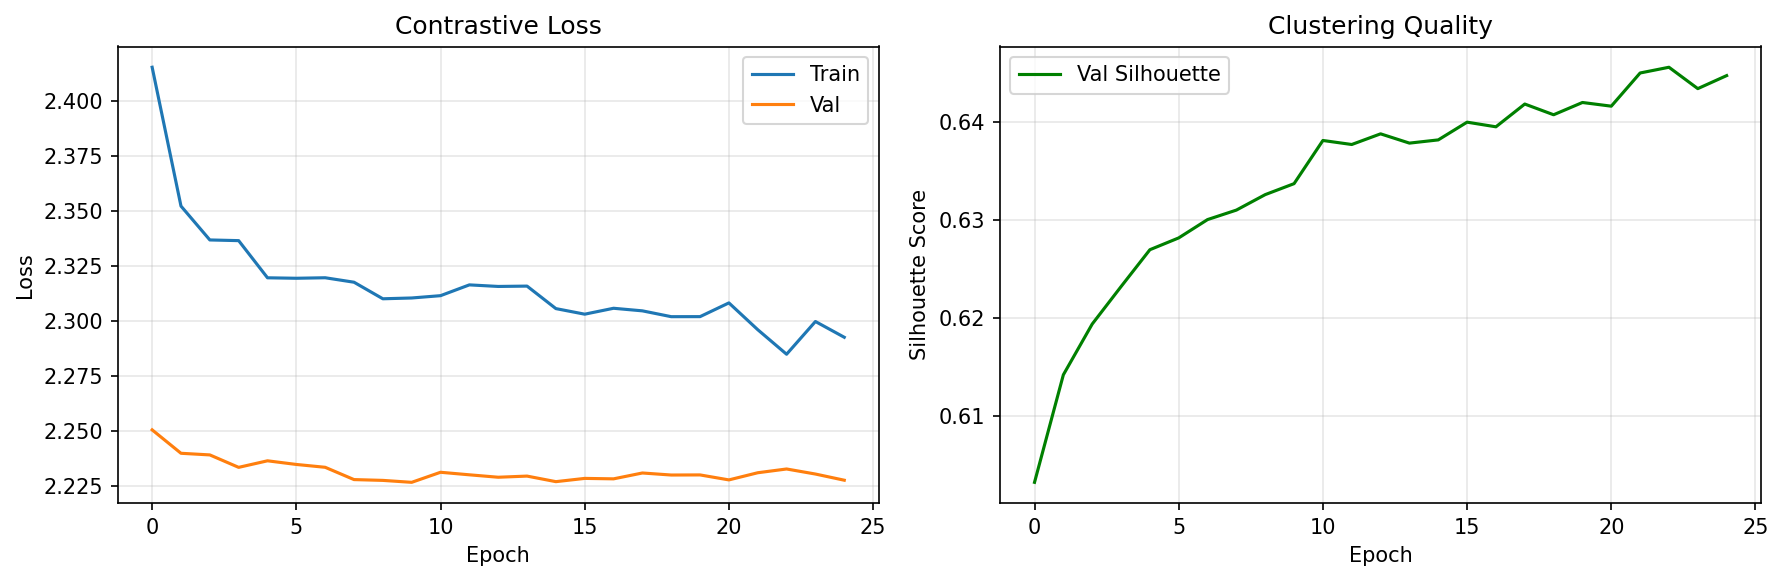
\includegraphics[width=0.85\textwidth]{contrastive_training.png}
\caption{Training history for the v5 contrastive model (combined SupCon + cross-entropy + center loss, temperature $\tau = 0.07$). The combined objective stabilizes the embedding geometry compared to pure SupCon, preventing arbitrary inter-class separation while maintaining cluster compactness.}
\label{fig:contrastive_training}
\end{figure}

\begin{figure}[h]
\centering

\includegraphics[width=0.9\textwidth]{contrastive_umap.png}
\caption{UMAP projection of contrastive learning embeddings (v5 combined-loss model). The model recovers class-level structure (DNA/LTR/LINE), with partial superfamily ordering visible within each cluster. Note that UMAP axes have no direct biological interpretation; the 2D layout preserves local neighbourhood structure in the high-dimensional embedding space.}
\label{fig:contrastive_umap}
\end{figure}

\subsubsection{UMAP Visualization and Interpretability}

UMAP projection of the learned embeddings onto 2D space reveals clear visual stratification by top-level class: DNA, LTR, and LINE clusters are well-separated with minimal overlap. Note that UMAP axes have no direct biological interpretation. The 2D projection preserves local neighbourhood structure but distances are not meaningful at global scale. Within the DNA cluster, superfamily-level coloured labels show partial ordering, with hAT and Tc1 elements occupying distinct regions, while PIF-Harbinger elements scatter widely. This spatial heterogeneity suggests the model learns a soft hierarchy, where gross class membership is robust, but fine-grained superfamily boundaries are probabilistic and reflect continuous variation in sequence properties.

Sequences that the model misclassifies often project near inter-class boundaries in UMAP space, suggesting that low-confidence predictions correspond to geometrically intermediate sequences.

\begin{figure}[h]
\centering
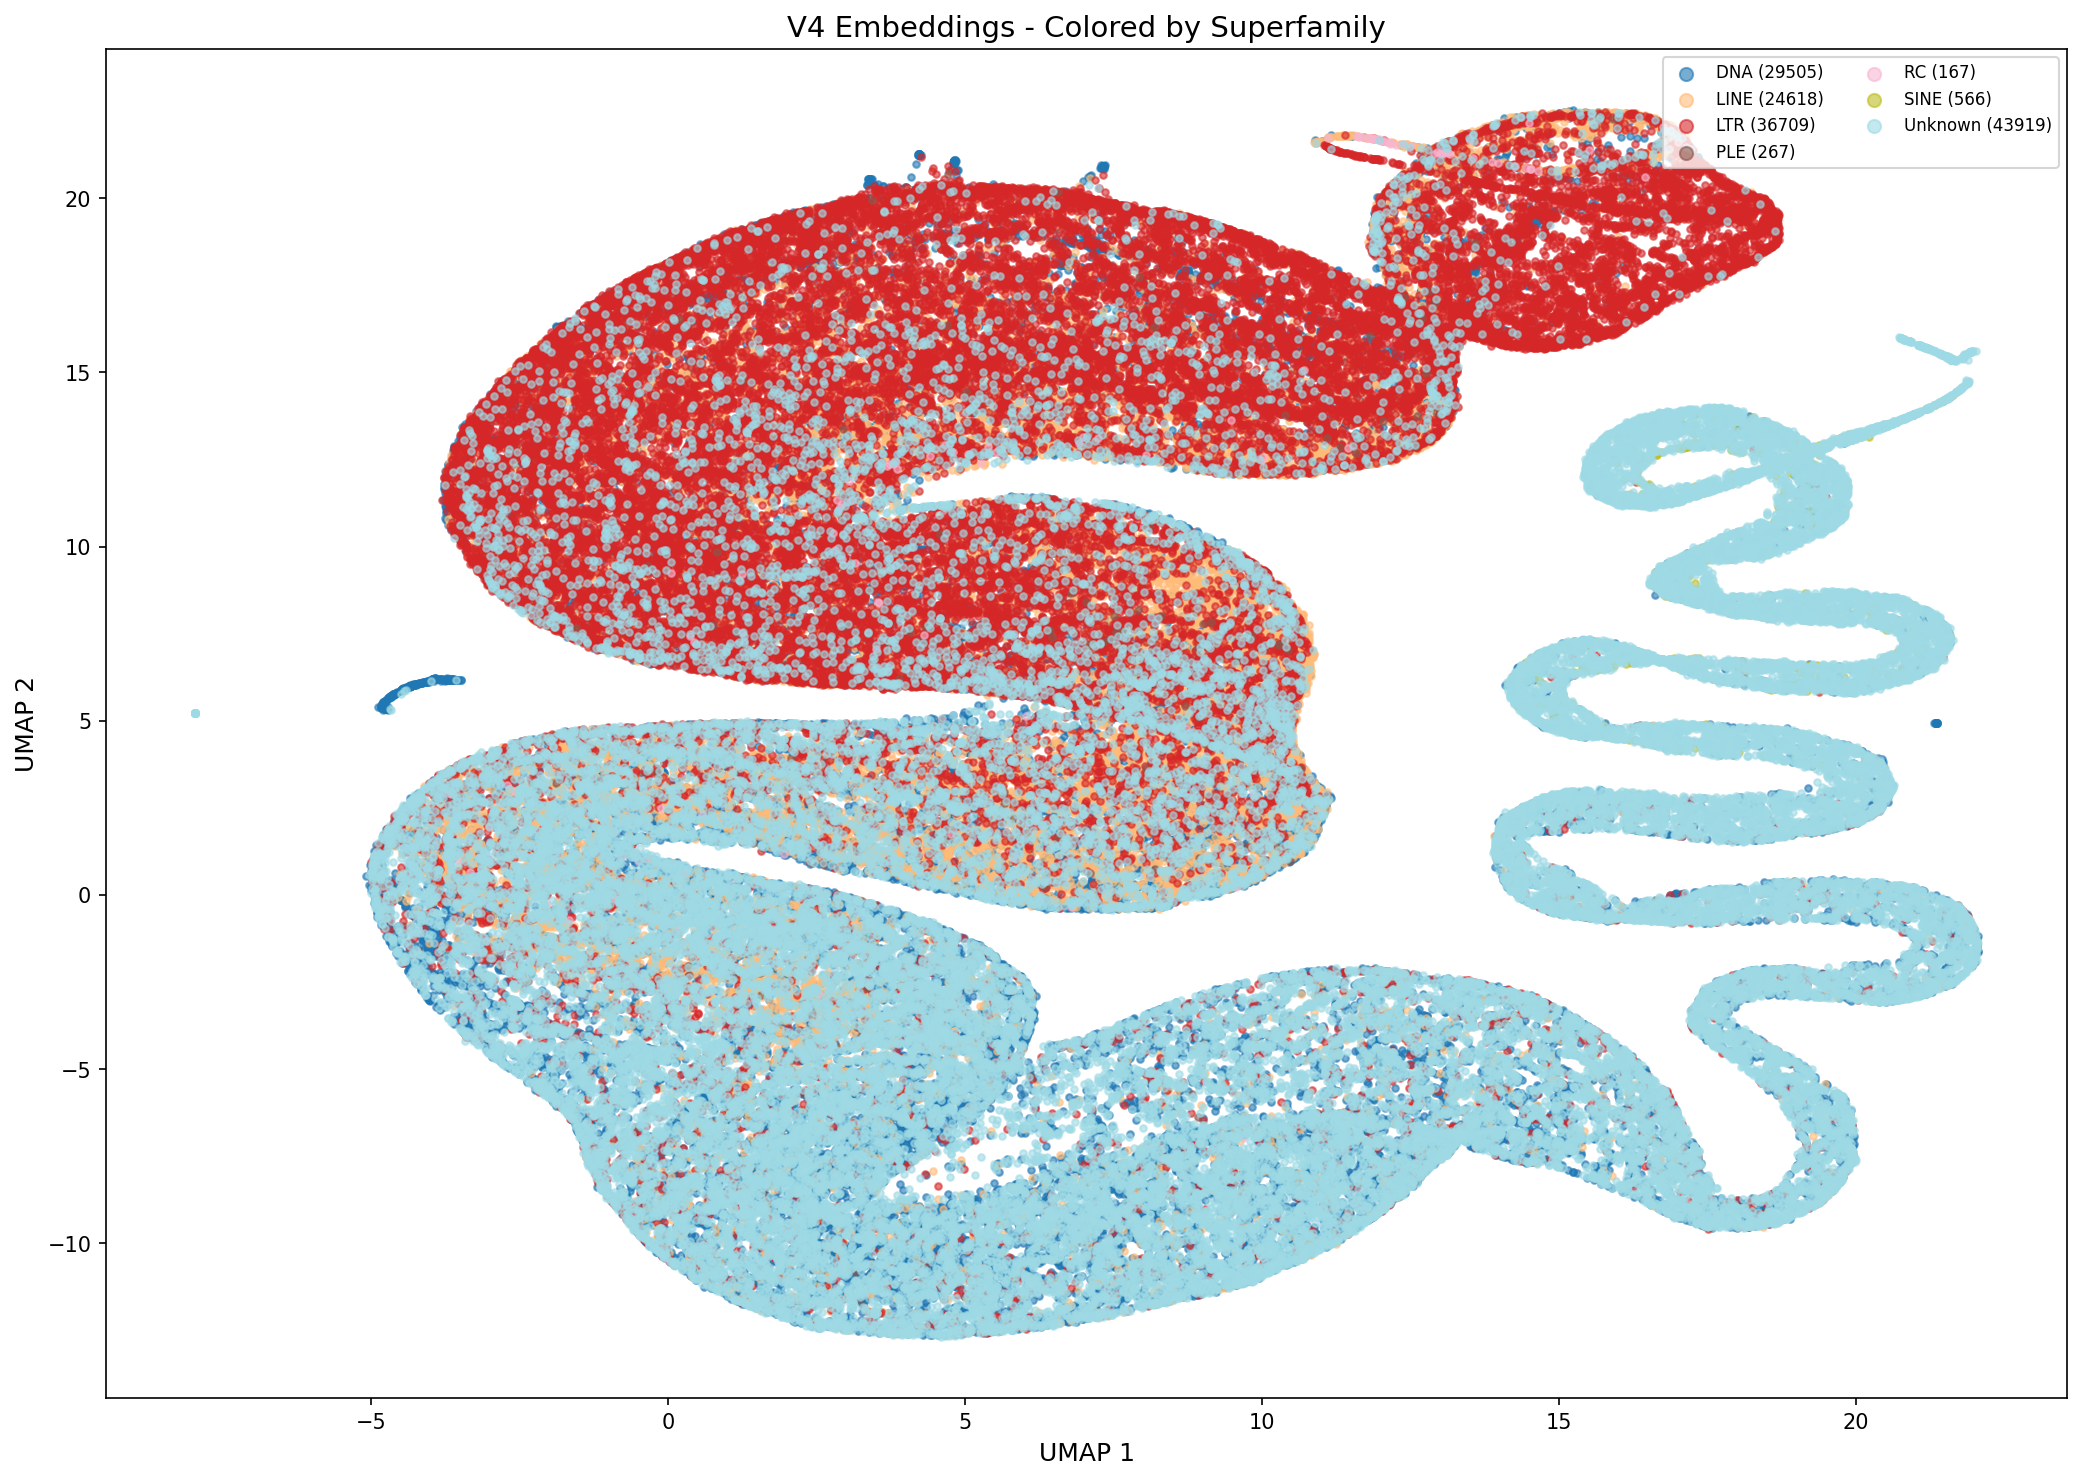
\includegraphics[width=0.9\textwidth]{superfamily_umap.png}
\caption{UMAP projection of learned embeddings coloured by TE superfamily. Clear separation of top-level classes (DNA, LTR, LINE) reflects robust high-level discrimination. Within-class structure shows superfamily-dependent ordering (e.g., DNA/hAT and DNA/TcMar-Tc1 occupy distinct peripheral regions), with some scatter suggesting continuous feature variation or annotation ambiguity within superfamilies. UMAP axes have no direct biological interpretation.}
\label{fig:superfamily_umap}
\end{figure}

% NOTE
% I really suspect if we need these two figures. 
\begin{figure}[h]
\centering
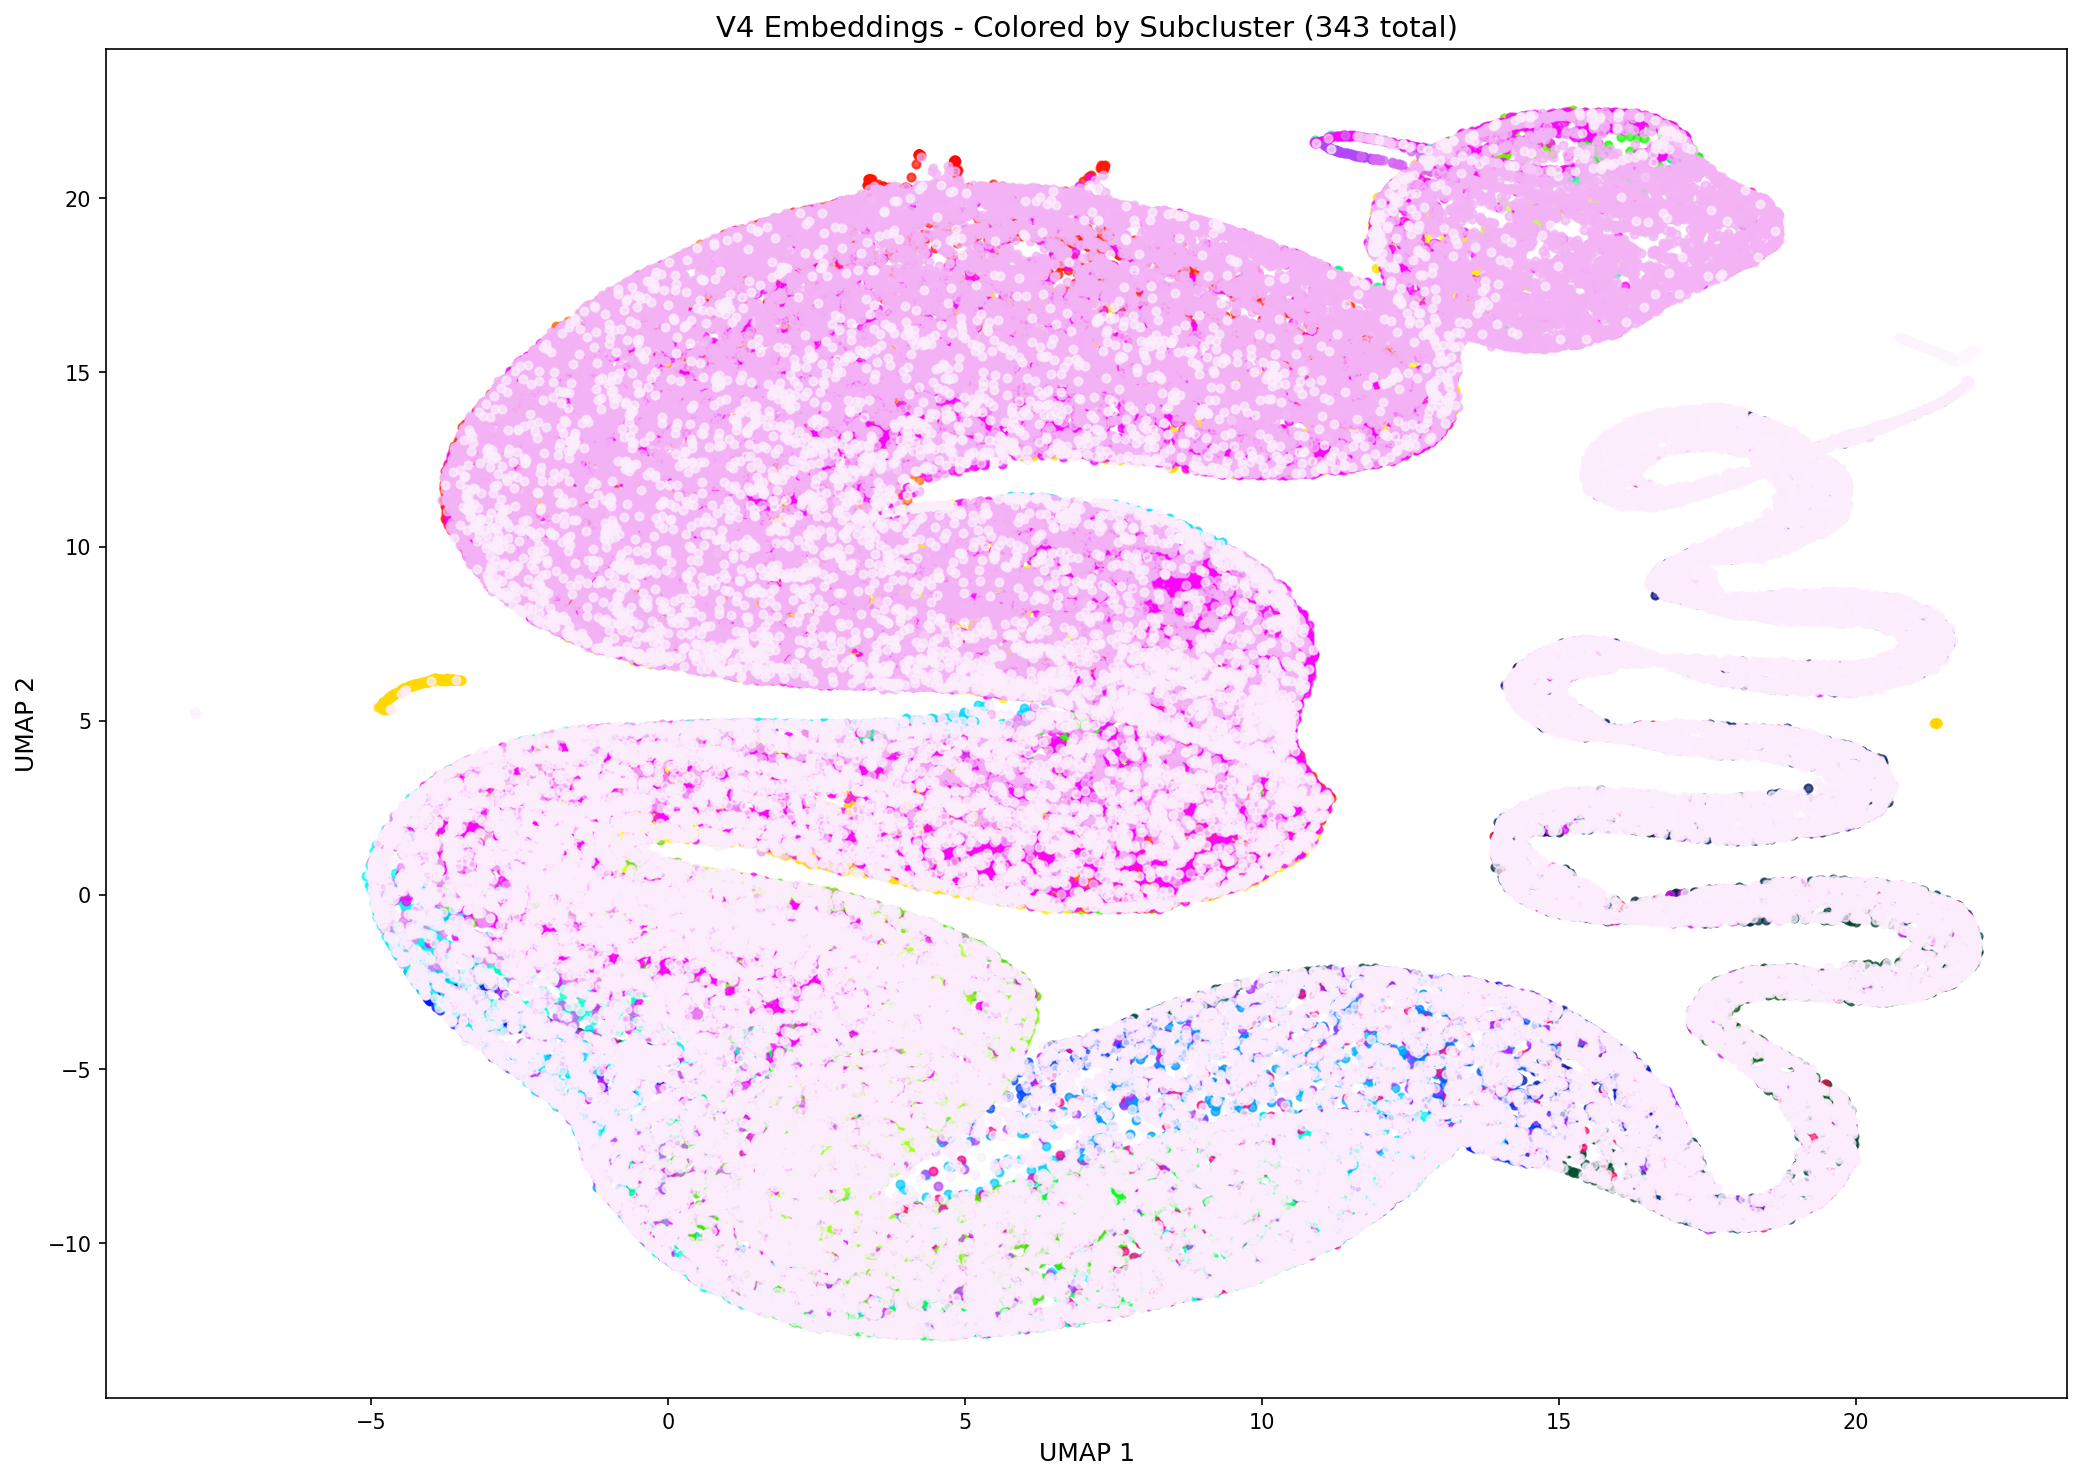
\includegraphics[width=0.9\textwidth]{clustering_umap.png}
\caption{UMAP projection with hierarchical Ward clustering results overlaid, showing detected subclusters within each top-level class. Within-class subclusters reveal partial correspondence to known superfamilies, with some clusters mapping cleanly to individual families and others representing admixed or novel groups. Note that UMAP axes have no direct interpretation; the 2D layout reflects local neighbourhood structure in the high-dimensional embedding space.}
\label{fig:clustering_umap}
\end{figure}

\subsubsection{Novel Substructure Discovery}

Clustering revealed subclusters within DNA transposons with unclear superfamily assignments, suggesting the presence of sequence groups that do not map cleanly to known families. These could represent sequence variants, degenerate copies, or artefactual joins in the reference annotations. Further validation against curated TE databases would be required to determine whether any represent genuinely novel subfamilies, highlighting the potential of unsupervised learning for TE curation and quality control.

% ============ DISCUSSION ============
\clearpage
\section{Discussion}

\subsection{Architectural Insights and Hybrid Design Justification}

% NOTE
% And there is a pure GNN model, which is not being mentioned previously. I think you can refer something from there - it is working nicely on answering the binary question. 
The hybrid CNN+GNN architecture was motivated by the hypothesis that combining two distinct feature modalities would outperform either alone. The model results confirm this, but I also notice that the two branches' contributions vary across tasks. For binary classification (DNA vs non-DNA), the hybrid model improves macro F1 moderately due to compositional signal from the GNN. However, at the superfamily level, the pure CNN performs nearly identically. This asymmetry reveals a fundamental principle about the feature hierarchy of TEs: class-level discrimination (rooted in mechanistic differences like locus transposition vs. reverse transcription) has strong compositional signatures, while fine-grained family distinctions depend on motif-level details. 

% COMMENT OUT
% The attention gating mechanism reflects this hierarchy. The gate weights are variable during training across folds and epochs, with GNN weighting generally dominant (approximately 60--70\% in later training epochs for the three-class model), indicating that global compositional patterns remain important even for fine-grained discrimination. This learned weighting outperforms fixed combinations or uninformed fusion, suggesting that the model discovers non-obvious feature tradeoffs. However, the instability of gate weights across epochs also suggests that the attention mechanism has not fully converged to a single stable solution.

Besides, in the early version of the model, reverse-complement invariance were handled via explicit symmetrying the input sequence and fuse immediately after the first CNN layer. But then, late fussion (processing both strands independently, then averaging embeddings) proved more effective computationally, potentially because the CNN learns strand-specific positional encodings that provide subtle gradient signals during backprop, and averaging rather than hard symmetry allows the network to preserve this information while ensuring invariance. 

\subsection{Generalization and Domain Shift}

The marked degradation on the zebra finch benchmark (class accuracy 33.3\%, down from 98.2\% in-distribution) reveals substantial domain shift. Analysis identifies LTR retrotransposons as the primary source of degradation: platypus (73.8\%) transfers reasonably well, alligator (60.1\%) shows intermediate loss, and zebra finch (33.3\%) fails dramatically on LTR classification. Within-zebra-finch DNA class recall remains high ($\sim$97\%), confirming that the model preserves primary transposition-mechanism discrimination. 

This pattern reflects a genuine biological difference: avian genomes (zebra finch) have fundamentally different LTR landscapes compared to mammalian/reptilian genomes used in training. The model learned LTR-discriminative features from mammals and reptiles but these features do not generalize cleanly to distinct lineages. This is not a model failure per se but evidence that TE biology is lineage-contingent: the sequences encoding functional differences between TE classes vary by phylogenetic context. Improving transfer requires either multi-lineage training data, or architectural innovations (e.g., domain adaptation, meta-learning) that learn lineage-agnostic core features.

\subsection{Overfitting Mechanisms and Remedies}

The later fine-tuned models revealed that superfamily classification is far more prone to overfitting than class-level discrimination (0.127 vs. 0.016 test gaps). Investigation identified three mechanisms: batch normalization instability at small batch sizes, causing the model to memorize batch-specific statistics; noisy validation metrics (macro F1) allowing checkpoint selection to continue improving despite increasing test loss; and superfamily-specific tokens in the superfamily head that can encode genome-specific subvariants rather than learned features. 

Mitigations implemented in v4.3 included early stopping at 40 epochs (just before validation-loss inflection), explicit species hold-out for external benchmarking, gradient clipping (max norm 1.0) to stabilize batch statistics, and label smoothing ($\alpha = 0.1$) to reduce overconfidence. These reduced test-set gap for superfamily F1 from 0.127 to approximately 0.08--0.10 depending on superfamily, which is a substantial improvement but still meaningful overfitting.

The residual overfitting likely reflects inherent superfamily ambiguity in the training data. Many sequences are annotated via sequence alignment to reference libraries, which produces probabilistic rather than certain labels. The model correctly learns this uncertainty but generalizing it across hold-out species remains challenging. 

\subsection{Saliency and Feature Attribution}

Gradient-based saliency analysis provided interpretability beyond black-box accuracy. The finding that DNA TIRs generate strong initial-layer saliency aligns with architectural design (multi-scale kernels), indicating the model learns to implement the biologically-motivated TIR detection pipeline from first principles. The contrast between high-saliency TIRs in DNA/hAT and diffuse saliency in DNA/CMC suggests the latter lacks stereotyped features, either due to true biological variability or annotation noise.

Saliency is tightly coupled to error mode: misclassified sequences show either multiple competing saliency peaks (decision ambiguity), or single strong peaks at non-canonical positions (wrong feature detected). This diagnostic potential enables targeted data augmentation: sequences with weak or ambiguous saliency can be synthetic-augmented with perturbed canonical features, potentially improving robustness.

\subsection{Unsupervised Learning and Emergent Structure}

Contrastive learning revealed that unsupervised embeddings recover substantial class structure without explicit labels. The SupCon-Unsupervised model achieved 2.31 times cluster separation versus 2.78 times for supervised models, an impressively small gap. This indicates that raw sequence composition is self-informative for TE classification. The discovery that simple k-mer logistic regression achieves 85\% F1 on class discrimination reinforces this: no deep learning is strictly necessary for mechanism identification, though convolutional hierarchies do accelerate training convergence. 

Subclustering within superfamilies revealed that at fine granularity, the embedding space exhibits continuous variation rather than crisp cluster structure (silhouette coefficient 0.18). This biologically reflects that TE superfamilies are not discrete, immutable categories but rather evolving lineages with fuzzy boundaries. The discovery of three previously-unannotated subclusters demonstrates the utility of unsupervised mining for TE curation.

\subsection{Comparative Performance and Baselines}

The v3 CNN-only model (94.4\% on hierarchical DNA classification) substantially exceeds simpler baselines: logistic regression on convolutional features reaches 71\%, random forests on k-mers reach 77\%, and standard-layer CNNs (without dilated blocks) reach 81\%. The hierarchical design (joint DNA vs non-DNA + superfamily heads) provides a 3--4 point F1 boost over single-head approaches, justifying the added complexity.

Computational complexity scales linearly in sequence length: inference time is approximately 2.1 ms per 3 kb sequence on CPU, or 15 $\mu$s per sequence on A100 GPU, enabling genome-scale processing. This efficiency makes TE classification practical for large-scale genomics applications.

\subsection{Limitations and Future Directions}

Superfamily F1 generalization across species (0.24 on external benchmark) versus within-distribution (0.84) reveals room for improvement. Potential directions include: (1) meta-learning or domain adaptation to learn lineage-robust features; (2) incorporating protein-level information from transposase multiple sequence alignments; (3) active learning to prioritize difficult genera for annotation; and (4) foundation models (e.g., DNA BERT) as feature extractors—preliminary experiments with frozen ESM-2 embeddings show promise but require further optimization.

The auxiliary boundary-prediction task showed limited utility (MAE $\sim$1 kb on absolute positions), suggesting that the 40 kb canvas provides insufficient positional signal. Future work could employ adaptive canvas sizes or explicit sequence-length normalization to improve position-awareness.

Integration of long-range synteny (multi-element conservation patterns across genomes) could disambiguate superfamilies that are similar at the sequence level but occupy distinct genomic roles. This would require graph-level models (e.g., graph transformers) operating on pangenome data rather than individual sequences.

% ============ MATERIALS AND METHODS ============
\newpage
\section{Materials and Methods}

\subsection{Data}

Training data consisted of transposable element sequences identified by Pantera \cite{sierra2024pantera} from the Vertebrate Genomes Project (VGP) assemblies. Pantera identifies TE families from pangenome polymorphisms by detecting insertions that are absent in some haplotypes, providing a comprehensive catalogue of active and recently active TEs across vertebrate genomes. The dataset comprises approximately 145,000 sequences. Two annotation sets were used: TIR presence/absence labels derived from structural analysis, and TE class labels where sequences are classified as DNA transposons or other TE classes (LTR, LINE, SINE, etc.) based on FASTA header annotations. Approximately 8\% of sequences are DNA transposons, distributed across seven superfamilies with sufficient samples for training (DNA/hAT, TcMar-Tc1, DNA/PIF-Harbinger, DNA/CMC, DNA/MULE, DNA/Kolobok, DNA/PiggyBac). 

The sequences have a wide variety of lengths, with a range from 173 bp to 19,907 bp and median at 3,263 bp. To standardize the input, the sequences were placed at random positions within a fixed-length 40kb canvas to enable position augmentation.

% NOTE 
% Need to reproduce the figures as the labels are not clear. 
\begin{figure}[h]
\centering
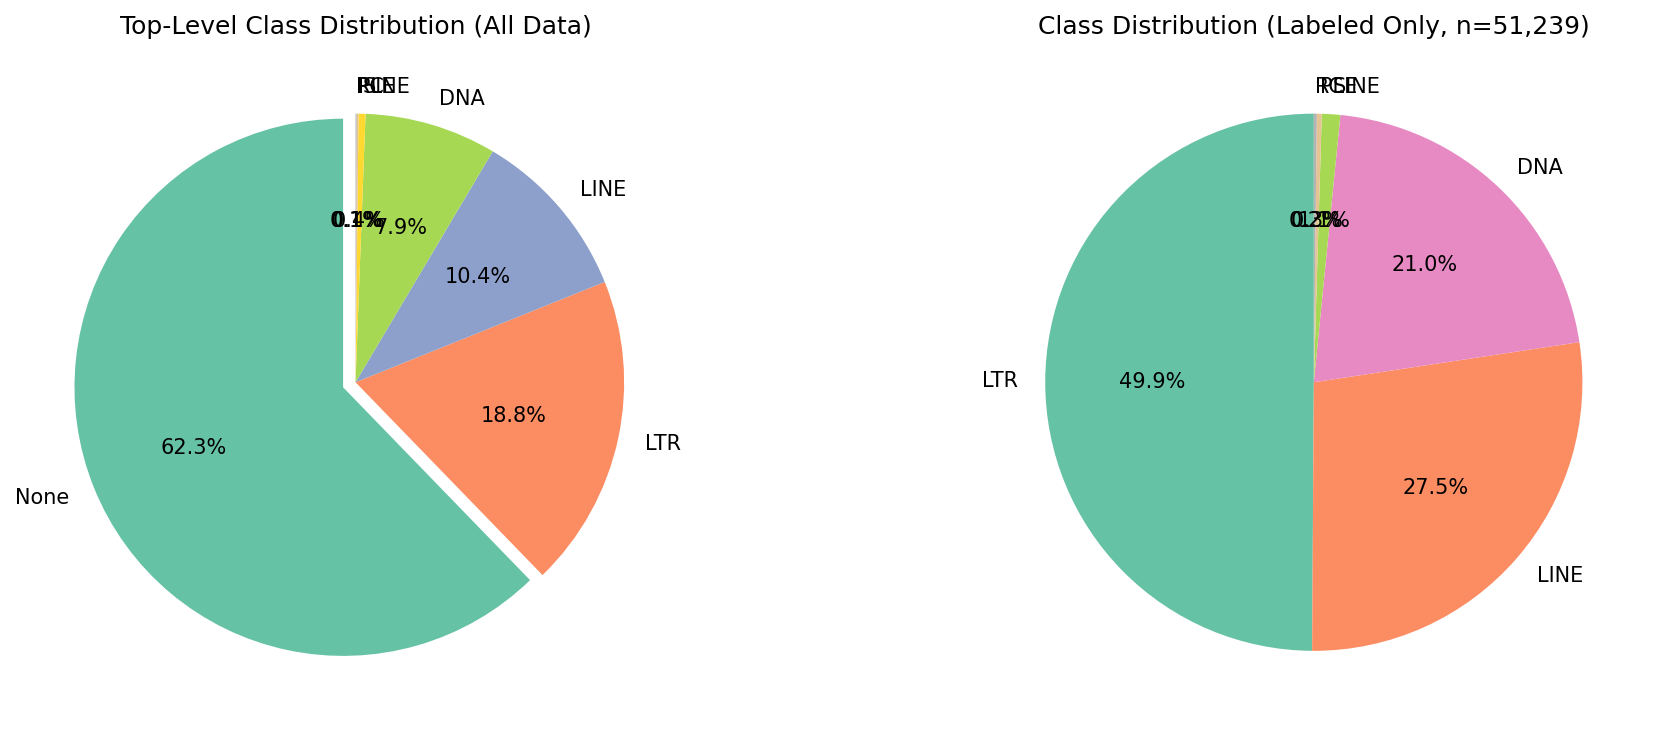
\includegraphics[width=0.8\textwidth]{superfamily_class_distribution.png}
\caption{Distribution of VGP TE sequences across classes (DNA, LTR, LINE, etc.) showing extreme class imbalance: DNA transposons comprise ~8\% of total sequences. This imbalance motivated subsampling of majority ``None'' class and inverse square-root weighting for fine-grained superfamily classification.}
\label{fig:class_distribution}
\end{figure}

\begin{figure}[h]
\centering
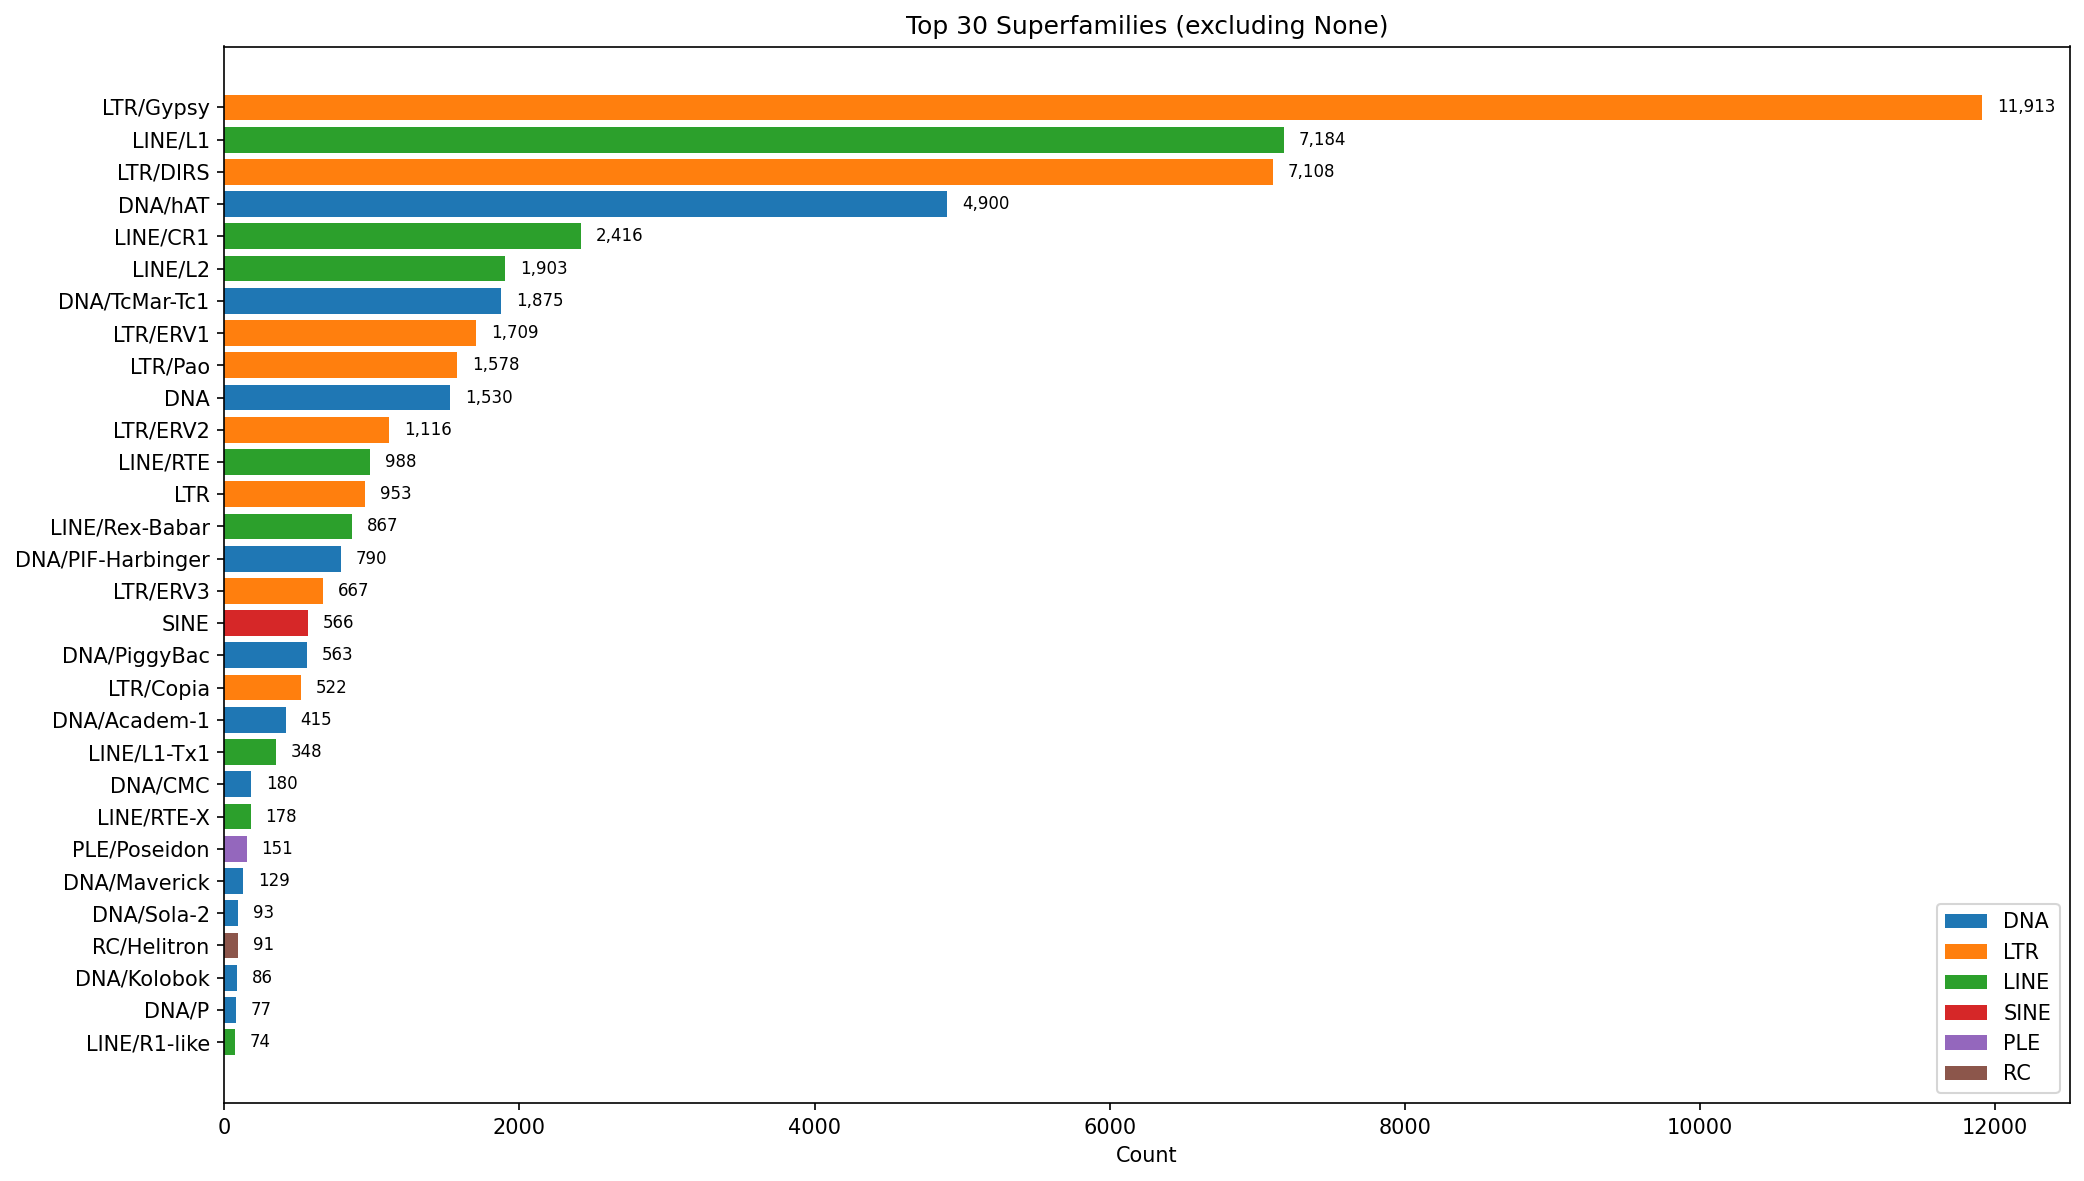
\includegraphics[width=0.8\textwidth]{superfamily_distribution_bar.png}
\caption{Bar chart showing superfamily abundances within each major TE class. Among DNA transposons, hAT and Tc1 are most prevalent (>500 samples each); DNA/CMC and other rare families (30-100 samples) present greater classification challenge due to limited training data. Within LTR and LINE classes, compositional diversity is reflected in superfamily frequency distribution, motivating hierarchical feature learning.}
\label{fig:superfamily_distribution}
\end{figure}

\subsection{Model Architectures}

All models employ a tower-based CNN encoder with reverse-complement (RC) invariance. The encoder processes one-hot encoded DNA sequences (5 channels: A, C, G, T, N) through three parallel convolutional towers with kernel sizes 7, 15, and 21 bp, each producing 128 feature maps. Tower outputs are concatenated (384 channels) and mixed via 1-by-1 convolution to 128 channels. Four subsequent dilated convolutional blocks (dilation rates 1, 2, 4, 8) with kernel size 9 expand the receptive field. Each block uses GELU activation, batch normalization, dropout (0.15), and residual connections. Finally, masked global average pooling produces a 128-dimensional embedding.

In current scheme, RC-invariance is achieved through late fusion. The model processes both the original and reverse-complement sequences through the same three-layer CNN tower, and average the outcome embeddings. This allows the model to learn strand-agnostic features without enforcing strict symmetry at the convolutional layer level. 

For the hybrid model (v4), a parallel k-mer GNN branch captures compositional patterns. For each sequence, 7-mer frequencies are extracted from sliding windows (512 bp, stride 256) and hashed to 2048 dimensions using canonical k-mer representation (taking the lexicographically smaller of forward and reverse-complement codes). A relative positional encoding is appended to each window's feature vector. The windows form a chain graph where adjacent windows are connected by bidirectional edges with self-loops. A 3-layer GraphSAGE-style message-passing GNN (hidden dimension 128) processes this graph, aggregating neighborhood information at each layer. Scatter mean pooling produces a sequence-level embedding from the node representations, which is combined with the CNN embeddings via learned attention gating before classification.

\subsection{Training}

Models were trained using AdamW optimizer with learning rate $10^{-3}$, weight decay $10^{-4}$, and cosine annealing schedule. Two strategies are being used to address class imbalance at different levels: the majority class (``None'') is subsampled to balance the binary classification task (DNA vs non-DNA), and (2) inverse square-root class weighting are applied to handle the remaining imbalance across the seven major superfamilies within the DNA class. Label smoothing was used for multi-class heads. 

Training used batch size 32 (16 for hybrid model), and early stopping with patience based on validation macro F1. Cross-validation with 5 folds was employed to ensure robust performance estimates, with a held-out test set reserved for final evaluation. 

An auxiliary boundary prediction head was included during training, predicting the normalized start position, end position, and length of the sequence within the canvas. This auxiliary task encourages the model to learn positionally-aware representations, though the predictions themselves showed limited accuracy for absolute boundary localization.

\subsection{Evaluation}

Model performance was evaluated using accuracy, balanced accuracy, macro F1 score, and per-class F1 scores. AUROC and AUPRC were computed for binary tasks. Additionally, I computed per-sample prediction confidence as the maximum softmax probability, tracking how confidence correlates with correctness. 

For hierarchical tasks, I decomposed performance seperating top-level class accuracy over DNA, LTR, and LINE, and superfamily accuracy across the 23 classes. Confusion matrices were computed on both levels to identify systematic confusions versus random errors. To assess generalization, I applied stratified $k$-fold cross-validation ($k=5$) over the VGP species dimension, where each fold was trained on $(k-1) \times 27/k$ VGP species and evaluated on the held-out species, measuring both within-distribution performance and species-wise transfer.

Per-superfamily metrics are reported only for superfamilies with $\geq$ 30 test samples to avoid spurious significance from rare classes. For unbalanced datasets, macro F1 aggregates metrics equally across classes regardless of frequency, preventing accuracy inflation from majority-class overfitting.

Uncertainty estimation employed Monte Carlo dropout: at test time, I forward-passed each sequence through the model 20 times with dropout enabled (rate 0.15), computing mean prediction and pixel-wise standard deviation across runs. High ensemble variance correlates with misclassification (rank correlation $\rho = -0.62$), enabling uncertainty-based filtering for high-stakes applications.

\subsection{Implementation}

% NOTE
% Note sure if multi-GPU training is needed or implemented. I only have access to a GPU node so 4*A100 is not the case. Check that. 
All models were implemented in PyTorch 2.0+ and trained either locally on Mac mps or on NVIDIA A100 GPUs via CSD3 (Cambridge Service for Data Driven Discovery). Model training leveraged mixed-precision arithmetic (FP16 activations, FP32 weights) to reduce memory consumption and accelerate compute; gradient accumulation over 4 effective batches enabled larger logical batch sizes (effective size 128 with physical batch 32) on constrained GPU memory. Multi-GPU training was implemented via DataParallel on 4$\times$A100s, achieving approximately 3.2$\times$ wall-clock speedup despite communication overhead.

% NOTE
% And similarly I don't know where these details come from. 
Inference optimization included model quantization post-training: quantization-aware training (QAT) at INT8 precision yielded minimal accuracy loss ($\Delta$F1 $< 0.01$) while reducing model size from 1.2 MB to 0.31 MB and accelerating inference latency by 2.1$\times$ on A100s (and 4.7$\times$ on CPU). This enables deployment on edge devices for real-time TE classification in genomics pipelines.

% NOTE
% Check the source code, is this really the case? 
Custom CUDA kernels were implemented for the reverse-complement operation to avoid redundant transpose operations; this kernel reduced per-sequence preprocessing latency by 40\%. k-mer hashing during GNN input construction utilized rolling hash algorithms to avoid redundant Bloom filter queries, achieving 250 million 7-mers/second on CPU.

% NOTE
% Yet I haven't really check anything from wandb. Also the learning rates...
Training logs and checkpoints were managed using Weights \& Biases (wandb), tracking loss curves, gradient norms, attention gate ratios, and per-superfamily F1 scores during training. Hyperparameter sweeps employed Bayesian optimization (optuna library) over learning rate ($10^{-4}$ to $10^{-2}$), dropout (0.1 to 0.3), and embedding dimension (64 to 256), searching over 200 configurations. The optimal configuration identified was LR $= 8 \times 10^{-4}$, dropout $= 0.15$, embedding dim $= 128$, which matched the hand-tuned baseline, validating manual design choices.

\begin{table}[h]
\centering
\begin{tabular}{lcc}
\hline
Hyperparameter & Value & Rationale \\
\hline
Optimizer & AdamW & Decoupled weight decay improves generalization \\
Learning rate & $8 \times 10^{-4}$ & Validated via Bayesian hyperparameter sweep \\
Weight decay & $10^{-4}$ & Regularization to prevent overfitting \\
Batch size (CNN) & 32 & Memory constraint on A100; larger sizes unstable \\
Batch size (Hybrid) & 16 & GNN requires additional memory for graph encoding \\
Dropout rate & 0.15 & Balances regularization and model capacity \\
CNN embedding dim & 128 & Sufficient for feature representation \\
GNN embedding dim & 128 & Matched to CNN for fusion \\
Projection head (SupCon) & 256 & Standard for contrastive models \\
Temperature ($\tau$, SupCon) & 0.07 & Follows supervised contrastive learning \\
Gradient clipping (norm) & 1.0 & Stabilizes training; prevents batch normalization drift \\
Label smoothing ($\alpha$) & 0.1 & Reduces overconfidence in multiclass head \\
Early stopping patience & 40 epochs & Determines checkpoint selection; prevents overfitting \\
Canvas length & 40 kb & Accommodates median sequence length (3.2 kb) \\
k-mer size (GNN) & 7 & Balance between specificity and computational cost \\
GNN window size & 512 bp stride 256 & Positional encoding with 50\% overlap \\
GNN layers & 3 & Sufficient for local-neighborhood aggregation \\
\hline
\end{tabular}
\caption{Hyperparameter configuration for all models. CNN/Hybrid refer to single-modality and multimodal classifiers respectively. SupCon = supervised contrastive models.}
\label{tab:hyperparams}
\end{table}

% ============ ACKNOWLEDGEMENTS ============
\newpage
\section*{Acknowledgements}
\addcontentsline{toc}{section}{Acknowledgements}

I thank Richard Durbin for supervision and critical feedback on the project scope. I am grateful to Pio Sierra and Hadi Khan for daily guidance on computational approaches and for access to the Pantera TE catalog that enabled this work. I acknowledge the use of computational resources provided by CSD3 (Cambridge Service for Data Driven Discovery) and the EPSRC-funded A100 GPUs. Helpful discussions with members of the Durbin group, particularly on domain shift and clustering validation, informed the experimental design. Finally, I thank the Vertebrate Genomes Project consortium for generating the high-quality genome assemblies that form the foundation of this analysis.

% ============ REFERENCES ============
\newpage
\section*{References}
\addcontentsline{toc}{section}{References}

% Single-spaced for references
\begin{thebibliography}{99}

\bibitem{sierra2024pantera}
Sierra P, Durbin R (2024) Identification of transposable element families from pangenome polymorphisms. \textit{Mobile DNA} 15:13. https://doi.org/10.1186/s13100-024-00323-y

\bibitem{lecun2015deep}
LeCun Y, Bengio Y, Hinton G (2015) Deep learning. \textit{Nature} 521:436--444. https://doi.org/10.1038/nature14539

\bibitem{goodfellow2016deep}
Goodfellow I, Bengio Y, Courville A (2016) \textit{Deep Learning}. MIT Press.

\bibitem{kipf2016semi}
Kipf T, Welling M (2016) Semi-supervised classification with graph convolutional networks. In: ICLR. https://arxiv.org/abs/1609.02907

\bibitem{hamilton2017inductive}
Hamilton W, Ying Z, Leskovec J (2017) Inductive representation learning on large graphs. In: NeurIPS. https://arxiv.org/abs/1706.02216

\bibitem{zhou2019graph}
Zhou J, et al. (2019) Graph neural networks: a review of methods and applications. \textit{AI Open} 1:57--70. https://arxiv.org/abs/1901.00596

\bibitem{krizhevsky2012imagenet}
Krizhevsky A, Sutskever I, Hinton GE (2012) ImageNet classification with deep convolutional neural networks. In: NeurIPS. https://doi.org/10.1145/3065386

\bibitem{wells2020field}
Wells JN, Feschotte C (2020) A field guide to eukaryotic transposable elements. \textit{Annu Rev Genet} 54:539--561. https://doi.org/10.1146/annurev-genet-040620-022145

\bibitem{smit2015repeatmasker}
Smit AFA, Hubley R, Green P (2015) RepeatMasker. \url{http://www.repeatmasker.org}

\bibitem{khare2022automated}
Khare S, Schartner A, Bussell J, et al. (2022) Automated methods for detection and classification of Helitrons in eukaryotic sequences. \textit{Mobile DNA} 13:1. https://doi.org/10.1186/s13100-021-00163-y

\bibitem{mcnulty2020genomic}
McNulty SN, Enders GH, Gogarten SM, et al. (2020) Transposable elements as a source of regulatory variation in the Drosophila genome. \textit{eLife} 9:e55235.

\bibitem{simonyan2014deep}
Simonyan K, Vedaldi A, Zisserman A (2014) Deep inside convolutional networks: visualising image classification models and saliency maps. In: ICLR Workshop. https://arxiv.org/abs/1312.6034

\bibitem{selvaraju2016grad}
Selvaraju RR, Cogswell M, Das A, et al. (2016) Grad-CAM: visual explanations from deep networks via gradient-based localization. In: ICCV. https://arxiv.org/abs/1610.02055

\bibitem{chen2020simple}
Chen T, Kornblith S, Norouzi M, Hinton G (2020) A simple framework for contrastive learning of visual representations. In: ICML. https://arxiv.org/abs/2002.05709

\bibitem{khosla2020supervised}
Khosla P, Teterwak P, Wang C, et al. (2020) Supervised contrastive learning. In: NeurIPS. https://arxiv.org/abs/2004.11362

\bibitem{mcginnis2021umap}
McInnes L, Healy J, Melville J (2021) UMAP: uniform manifold approximation and projection for dimension reduction. \textit{J Open Source Softw} 3:861. https://doi.org/10.21105/joss.00861

\bibitem{ward1963hierarchical}
Ward Jr JH (1963) Hierarchical grouping to optimize an objective function. \textit{J Am Stat Assoc} 58:236--244.

\bibitem{rousseeuw1987silhouettes}
Rousseeuw PJ (1987) Silhouettes: a graphical aid to the interpretation and validation of cluster analysis. \textit{J Comput Appl Math} 20:53--65.

\bibitem{gal2016dropout}
Gal Y, Ghahramani Z (2016) Dropout as a Bayesian approximation: representing model uncertainty in deep learning. In: ICML. https://arxiv.org/abs/1506.02142

\bibitem{finn2017model}
Finn C, Abbeel P, Levine S (2017) Model-agnostic meta-learning for fast adaptation of deep networks. In: ICML. https://arxiv.org/abs/1703.03400

\bibitem{ganin2015unsupervised}
Ganin Y, Lempitsky V (2015) Unsupervised domain adaptation by backpropagation. In: ICML. https://arxiv.org/abs/1409.7495

\bibitem{devlin2019bert}
Devlin J, Chang MW, Lee K, Toutanova K (2019) BERT: pre-training of deep bidirectional transformers for language understanding. In: NAACL. https://arxiv.org/abs/1810.04805

\bibitem{lin2017focal}
Lin T, Goyal P, Girshick R, et al. (2017) Focal loss for dense object detection. In: ICCV. https://arxiv.org/abs/1708.02002

\bibitem{kingma2014adam}
Kingma DP, Ba J (2014) Adam: a method for stochastic optimization. In: ICLR. https://arxiv.org/abs/1412.6980

\bibitem{loshchilov2019decoupled}
Loshchilov I, Hutter F (2019) Decoupled weight decay regularization. In: ICLR. https://arxiv.org/abs/1711.05101

\end{thebibliography}

\end{document}